\documentclass[12pt]{report}
\usepackage[fontsize=13pt]{scrextend}
\usepackage[utf8]{vietnam}
\usepackage[utf8]{inputenc}
\usepackage[vietnamese]{babel}
\usepackage{titlesec}
\usepackage{titletoc}
\usepackage{listings}
\usepackage[bookmarks=true]{hyperref}
\usepackage[left=3cm,right=2cm,top=2.5cm,bottom=3cm]{geometry}
\usepackage{graphicx}
\usepackage{hyperref}
\usepackage{tikz}
\usepackage{varwidth}
\usepackage{float}
\usepackage{listings}
\usepackage{color}
\usepackage{multirow}
\usepackage{booktabs}
\usepackage[ruled,vlined]{algorithm2e}

\setlength{\parskip}{6pt}

\usetikzlibrary{calc}
\setlength{\parindent}{10mm}
\renewcommand{\baselinestretch}{1.3}
\graphicspath{{images/}}

\definecolor{dkgreen}{rgb}{0,0.6,0}
\definecolor{gray}{rgb}{0.5,0.5,0.5}
\definecolor{mauve}{rgb}{0.58,0,0.82}

% setup code area as listings
\lstset{frame=tb,
  language=Java,
  aboveskip=3mm,
  belowskip=3mm,
  showstringspaces=false,
  columns=flexible,
  basicstyle={\small\ttfamily},
  numbers=left,
  numberstyle=\tiny\color{gray},
  keywordstyle=\color{blue},
  commentstyle=\color{dkgreen},
  stringstyle=\color{mauve},
  breaklines=true,
  breakatwhitespace=true,
  tabsize=3
}

\renewcommand{\lstlistingname}{Mã nguồn}
\newenvironment{thuattoan}[1][h]
  {\renewcommand{\algorithmcfname}{Thuật toán}
   \begin{algorithm}[#1]
  }{\end{algorithm}}

% hyper setup
\hypersetup{
	bookmarks=true,
	pdftitle={Xây dựng công cụ hỗ trợ quản lý và đảm bảo chất lượng cho các phiên bản phần mềm},
	pdfauthor={Bùi Quang Cường}, % author
	pdfsubject={TeX and LaTeX},
	pdfkeywords={TeX, LaTeX, graphics, images}, % list of keywords
	colorlinks=true,       % false: boxed links; true: colored links
	linkcolor=blue,       % color of internal links
	citecolor=black,       % color of links to bibliography
	filecolor=black,        % color of file links
	urlcolor=purple,        % color of external links
	linktoc=page            % only page is linked
}

\date{}


\newpagestyle{long}
{\sethead{\thesection. \sectiontitle}{}{\subsectiontitle}\headrule
	\setfoot{}{\thepage}{}}

\begin{document}
\begin{titlepage}
	\center
	\begin{tikzpicture}[overlay,remember picture]
		\draw [line width=3pt,rounded corners=0pt,]
		($ (current page.north west) + (25mm,-25mm) $)
		rectangle
		($ (current page.south east) + (-15mm,25mm) $);
		\draw [line width=1pt,rounded corners=0pt]
		($ (current page.north west) + (26.5mm,-26.5mm) $)
		rectangle
		($ (current page.south east) + (-16.5mm,26.5mm) $);
	\end{tikzpicture}
	
	{\large \bfseries ĐẠI HỌC QUỐC GIA HÀ NỘI\\ TRƯỜNG ĐẠI HỌC CÔNG NGHỆ}\\[1cm]
	
\includegraphics[width=0.2\linewidth]{uet}\\[1cm]
	{\Large  \bfseries Bùi Quang Cường}\\[1.5cm]
	{ \LARGE \bfseries XÂY DỰNG CÔNG CỤ HỖ TRỢ QUẢN LÝ VÀ ĐẢM BẢO CHẤT LƯỢNG CHO CÁC PHIÊN BẢN PHẦN MỀM}\\[0.5cm]
	\hfill\\[1.5cm]
	{\large \bfseries KHÓA LUẬN TỐT NGHIỆP ĐẠI HỌC HỆ CHÍNH QUY}\\	
	{\large \bfseries Ngành: Công nghệ thông tin}	
	\hfill\\[3.5cm]	
	{\large \bfseries HÀ NỘI - 2018}\\	
	\vfill
\end{titlepage}
	
%-----SECONDARY TITLE PAGE-----%	
\begin{titlepage}
	\center
	\begin{tikzpicture}[overlay,remember picture]
		\draw [line width=3pt,rounded corners=0pt,]
		($ (current page.north west) + (25mm,-25mm) $)
		rectangle
		($ (current page.south east) + (-15mm,25mm) $);
		\draw [line width=1pt,rounded corners=0pt]
		($ (current page.north west) + (26.5mm,-26.5mm) $)
		rectangle
		($ (current page.south east) + (-16.5mm,26.5mm) $);
	\end{tikzpicture}
	
	{\large \bfseries ĐẠI HỌC QUỐC GIA HÀ NỘI\\ TRƯỜNG ĐẠI HỌC CÔNG NGHỆ}\\[2cm]

	{\Large  \bfseries Bùi Quang Cường}\\[2cm]		
	{ \LARGE \bfseries XÂY DỰNG CÔNG CỤ HỖ TRỢ QUẢN LÝ VÀ ĐẢM BẢO CHẤT LƯỢNG CHO CÁC PHIÊN BẢN PHẦN MỀM}\\[0.5cm]
	\hfill\\[1.5cm]
	{\large \bfseries KHÓA LUẬN TỐT NGHIỆP ĐẠI HỌC HỆ CHÍNH QUY}\\	
	{\large \bfseries Ngành: Công nghệ thông tin}
	\hfill\\[2cm]
	\begin{flushleft}
		{\large \bfseries Cán bộ hướng dẫn: PGS. TS. Phạm Ngọc Hùng}\\	
	\end{flushleft}
	\hfill\\[3cm]		
	{\large \bfseries HÀ NỘI - 2018}\\		
	\vfill		
\end{titlepage}

%-----TERTIARY TITLE PAGE-----%	
\begin{titlepage}
	\center
	\begin{tikzpicture}[overlay,remember picture]
	\draw [line width=3pt,rounded corners=0pt,]
	($ (current page.north west) + (25mm,-25mm) $)
	rectangle
	($ (current page.south east) + (-15mm,25mm) $);
	\draw [line width=1pt,rounded corners=0pt]
	($ (current page.north west) + (26.5mm,-26.5mm) $)
	rectangle
	($ (current page.south east) + (-16.5mm,26.5mm) $);
	\end{tikzpicture}
	
	{\large \bfseries VIETNAM NATIONAL UNIVERSITY, HA NOI\\ UNIVERSITY OF ENGINEERING AND TECHNOLOGY}\\[2cm]
	
	{\Large  \bfseries Bui Quang Cuong}\\[2cm]		
	{ \LARGE \bfseries BUILDING TOOL SUPPORTING FOR}\\[0.2cm]
	{ \LARGE \bfseries MANAGING AND QUALITY}\\[0.2cm]
	{ \LARGE \bfseries ASSURING OF SOFTWARE VERIONS}\\[0.5cm]
	\hfill\\[1.5cm]
	{\large \bfseries BACHELOR'S THESIS}\\	
	{\large \bfseries Major: Information Technology}
	\hfill\\[3cm]
	\begin{flushleft}
		{\large \bfseries Supervisor: Assoc. Prof., Dr. Pham Ngoc Hung}\\	
	\end{flushleft}
	\hfill\\[3cm]		
	{\large \bfseries HA NOI - 2018}\\		
	\vfill		
\end{titlepage}

%-----THANKS-----%
\newpage
\begin{titlepage}
\begin{center}
	\textbf{\large LỜI CẢM ƠN}
\end{center}
Đầu tiên, tôi xin gửi lời cảm ơn chân thành và sâu sắc tới thầy giáo PGS. TS. Phạm Ngọc Hùng – người đã trực tiếp hướng dẫn tận tình và đóng góp những ý kiến quý báu trong suốt quá trình tôi học tập, nghiên cứu cũng như khi tôi làm khóa luận tốt nghiệp này, người đã cho tôi nhiều lời động viên, những kiến thức quý báu giúp tôi trưởng thành hơn trong cuộc sống.

Tôi xin gửi lời cảm ơn tới những người bạn trong tập thể K59CLC – những người đã luôn đồng hành cùng tôi suốt bốn năm qua trên mọi nẻo đường, giúp đỡ tôi mỗi khi khó khăn, chia sẻ cùng tôi mọi chuyện trong học tập và cuộc sống và góp ý cho tôi những lời khuyên chân thành giúp tôi học tập tốt hơn và hoàn thành khóa luận này.

Tiếp theo tôi xin gửi lời cảm ơn đến các thầy cô giảng viên Trường Đại học Công Nghệ - Đại Học Quốc Gia Hà Nội – những người đã tận tâm truyền đạt những kiến thức quý báu làm nền tảng để tôi tiếp tục đi xa hơn nữa trong lĩnh vực công nghệ thông tin.Cuối cùng, tôi xin được cảm ơn cha mẹ, anh chị và người thân, những người đã không quản khó khăn, vất vả nuôi con ăn học để con có thể phấn đấu trở thành người có ích cho xã hội.
\end{titlepage}

	
%-----ABSTRACT-----%
\newpage
\begin{titlepage}
\begin{center}
	\textbf{\large TÓM TẮT}
\end{center}
\textbf{Tóm tắt:} Mã nguồn ứng dụng trở nên lớn và phức tạp sau quá trình dài phát triển, bảo trì và nâng cấp. Vấn đề này đang dần phổ biến đối với các doanh nghiệp phát triển phần mềm, gây khó khăn trong việc kiểm soát và đảm bảo chất lượng cho các ứng dụng. Hiện nay đã có một số công cụ được đề xuất để giải quyết vấn đề trên nhưng chưa có kết quả thỏa đáng. Nghiên cứu này đề xuất các phương pháp và xây dựng một bộ công cụ toàn diện cho việc phân tích và đảm bảo chất lượng mã nguồn cho các ứng dụng doanh nghiệp sử dụng các nền tảng J2EE phổ biến Struts 2, Hibernate, Spring. Đầu tiên, mã nguồn của ứng dụng sẽ được tiền xử lý để tạo cây cấu trúc. Mỗi nút trên cây đại diện cho một thành phần mã nguồn. Tiếp theo, các nút sẽ được phân tích theo các công nghệ sử dụng trong ứng dụng để xác định mối quan hệ phụ thuộc. Cây cấu trúc này được sử dụng làm đầu vào cho việc phân tích ảnh hưởng sự thay đổi và các chức năng phân tích cấu trúc như xây dựng đồ thị dữ liệu; xây dựng kiến trúc về công nghệ, cơ sở dữ liệu; tính toán độ phức tạp mã nguồn. Phương pháp phân tích ảnh hưởng sự thay đổi được đề xuất cải tiến theo hướng tự động hóa bằng phương pháp so sánh các phiên bản mã nguồn. Hiện nay, bộ công cụ đang được triển khai thử nghiệm tại Trung tâm công nghệ và quản lý chất lượng phần mềm Viettel (VITM) và nhận được nhiều phản hồi tích cực.\\

\noindent \textit{\textbf{Từ khóa:} phân tích mã nguồn, phiên bản mã nguồn, ứng dụng doanh nghiệp}
\end{titlepage}

%-----ABSTRACT (ENGLISH)-----%
\newpage
\begin{titlepage}
\begin{center}
	\textbf{\large ABSTRACT}
\end{center}
\end{titlepage}

%-----UNDERTAKING-----%
\newpage
\begin{titlepage}
\begin{center}
	\textbf{\large LỜI CAM ĐOAN}
\end{center}
Tôi xin cam đoan rằng những nghiên cứu về phương pháp hỗ trợ quản lý và đảm bảo chất lượng cho các phiên bản phần mềm được trình bày trong khóa luận này là của tôi và chưa từng được nộp như một báo cáo khóa luận tại trường Đại học Công Nghệ - Đại học quốc gia Hà Nội hoặc bất kỳ trường đại học khác. Những gì tôi viết ra không sao chép từ các tài liệu, không sử dụng các kết quả của người khác mà không trích dẫn cụ thể.Tôi xin cam đoan công cụ hỗ trợ quản lý và đảm bảo chất lượng tôi trình bày trong khoá luận là do tôi tự phát triển, không sao chép mã nguồn của người khác. Nếu sai tôi hoàn toàn chịu trách nhiệm theo quy định của trường Đại Học Công Nghệ - Đại Học Quốc Gia Hà Nội.\\

\begin{flushright}
	\begin{varwidth}{\linewidth}\centering
		Hà Nội, ngày 26 tháng 04 năm 2018\\
		Sinh viên\\[2cm]
		Bùi Quang Cường
	\end{varwidth}
\end{flushright}
\end{titlepage}

%-----TOC-----%
\newpage
\begin{titlepage}
\tableofcontents
\end{titlepage}

\newpage
\begin{titlepage}
\listoftables
\end{titlepage}

\newpage
\begin{titlepage}
	\listoffigures
\end{titlepage}

%-----MAIN-----%
\newpage
\setcounter{page}{1}
\chapter{Đặt vấn đề}
Hiện nay, các ứng dụng tại các doanh nghiệp thường được phát triển trong một thời gian
dài với quy mô lớn và độ phức tạp cao. Trải qua nhiều phiên bản nâng cấp, các ứng dụng
này thường thiếu tài liệu đặc tả và thiết kế. Có thể nói tài liệu gần như duy nhất của các
ứng dụng này là mã nguồn. Trong khi đó, quá trình bảo trì và nâng cấp diễn ra thường
xuyên. Để đảm bảo chất lượng cho mỗi phiên bản mới, đội dự án cần thực hiện kiểm thử
lại toàn bộ hệ thống. Điều này là không thể bởi chi phí cho việc này rất tốn kém. Kết quả
là chúng ta không thể kiếm soát toàn bộ sự ảnh hưởng của việc thay đổi và có thể dẫn đến
nhiều rủi ro lớn cho doanh nghiệp trong quá trình vận hành. Đây là một bài toán khó tổng
quát hóa vì các giải pháp đề xuất phụ thuộc chặt chẽ vào các công nghệ được sử dụng
trong ứng dụng. Đề xuất các giải pháp và xây dựng công cụ đủ tốt để giải quyết vấn đề
nêu trên đang là một trong những thách thức lớn và nhận được sự quan tâm nghiên cứu.

Phân tích ảnh hưởng sự thay đổi (Change Impact Analysis - CIA) được xem là một
giải pháp để giải quyết bài toán trên. CIA có vai trò quan trọng trong các giai đoạn phát
triển, bảo trì và kiểm thử hồi quy. Đối với người quản lý và lập trình viên, CIA là công cụ
đánh giá phạm vi ảnh hưởng, ước lượng chi phí từ đó lên kế hoạch thực hiện thay đổi.
Đối với kiểm thử viên, trong quá trình kiểm thử hồi quy, CIA có thể ứng dụng vào việc
xác định những ca kiểm thử có liên quan đến phần mã nguồn chỉnh sửa, điều này giúp
giảm số lượng các ca kiểm thử cần thực hiện từ đó rút ngắn thời gian và nỗ lực kiểm thử.
Các kĩ thuật CIA được thực hiện theo hai hướng tiếp cận chính là phân tích tĩnh (static
CIA) và phân tích động (dynamic CIA) [1]. Trong thực tế, hầu hết các nghiên cứu đề xuất
các phương pháp phân tích ảnh hưởng sự thay đổi liên quan đến static CIA. Nổi bật trong
số đó là kĩ thuật CIA dựa trên sự phân loại thay đổi [2], kĩ thuật dựa vào đồ thị Call
Graph [3] và kĩ thuật dựa trên tư tưởng giao thoa sóng nước WAVE-CIA [4]. Tuy nhiên,
Các kĩ thuật CIA sử dụng đầu vào là kết quả của quá trình phân tích phụ thuộc từ ứng
dụng. Quá trình này không thể tổng quát hóa cho toàn bộ các công nghệ và nền tảng hiện
có.

J2EE đang là một giải pháp phổ biến được sử dụng để triển khai cho các ứng dụng
Web doanh nghiệp hiện đại. Nó bao gồm nhiều công nghệ cốt lõi như EJB, JSF, CDI,
JAX-WS, JPA, JMS, v.v và có thể tích hợp nhiều framework khác như Spring, Struts,
Hibernate, Vaddin, GWT, Play!, Grails, v.v. Để giải quyết bài toán trên cho các ứng dụng 
2
J2EE, một phương pháp kèm theo công cụ có tên JCIA [5] đã được đề xuất và xây dựng.
Tuy nhiên phương pháp này khá thô sơ và chỉ đề xuất phân tích cho một số công nghệ cốt
lõi của J2EE. Công cụ JCIA còn đơn giản, chưa được hoàn thiện và chưa mang lại tính
hiệu quả cao.

Dựa trên ý tưởng về phương pháp này, một phương pháp hoàn chỉnh đã được nghiên
cứu và đề xuất để thực hiện phân tích ảnh hưởng sự thay đổi cho các ứng dụng J2EE đa
nền tảng. Các framework phổ biến hiện nay: Spring, Struts, Hibernate sẽ được tập trung
hỗ trợ đầu tiên. Sau đó chúng tôi sẽ dần hoàn thiện phương pháp cho các tất cả các nền
tảng khác. Ngoài ra, chúng tôi cũng đề xuất các giải pháp khác để đem lại nhiều góc nhìn
khách quan về hệ thống ứng dụng như xây dựng dòng dữ liệu, tái hiện thiết kế kiến trúc
hệ thống và cơ sở dữ liệu, và tính toán độ phức tạp mã nguồn. Một bộ công cụ được phát
triển như là phiên bản tiếp theo của công cụ JCIA để thực hiện các giải pháp đã đề xuất.

Các phần còn lại của báo cáo được cấu trúc như sau:
\begin{itemize}
\item Chương 2 - Lý thuyết về phân tích ảnh hưởng sự thay đổi. Chương này trình bày về lịch sử các kỹ thuật và quy trình chung phân tích ảnh hưởng sự thay đổi hiện nay.
\item Chương 3 - Phân tích ảnh hưởng sự thay đổi cho các ứng dụng J2EE. Trong chương này, một phương pháp về tiền xử lý mã nguồn ứng dụng J2EE để xây dựng cây cấu trúc sẽ được đề xuất. Bên cạnh đó, đề xuất các phương pháp để phân tích phụ thuộc cho Java Core và các framework J2EE. Cuối cùng là phương pháp phân tích ảnh hưởng sự thay đổi WAVE-CIA để áp dụng cho các ứng dụng J2EE.
\item Chương 4 - Phương pháp quản lý các phiên bản. Chương này mô tả cách quản lý các phiên bản mã nguồn dựa trên cây cấu trúc của mã nguồn.
\item Chương 5 - Thực nghiệm và triển khai. Chương này mô tả các kết quả thực nghiệm và đánh giá về các kết quả này.
\item Chương 6 - Kết luận. Kết luận của toàn bộ nghiên cứu và công cụ, trình bày các công việc tiếp theo cần thực hiện.
\end{itemize}


\newpage	
\chapter{Lý thuyết phân tích ảnh hưởng sự thay đổi}
Bảo trì phần mềm luôn được coi là hoạt động khó và tiêu tốn chi phí nhiều nhất trong quá trình phát triển phần mềm. Các sản phẩm phẩm phần mềm liên tục thay đổi và thích nghi với các yêu cầu thay đổi để phù hợp với nhu cầu của người dùng. Khi các thay đổi được thực hiện, nó sẽ gây ra các ảnh hướng không lường trước được, và có thể gây ra các tác động làm mất sự nhất quán đối với các thành phần của phần mềm.

Phân tích ảnh hưởng sự thay đổi (Change Impact Analysis - CIA) bao gồm một bộ các kỹ thuật giúp xác định sự ảnh hưởng của các thay đổi được đề xuất tới các thành phần phần mềm. Nó đóng vai trò quan trọng trong quá trình phát triển, bảo trì phần mềm và kiểm thử hồi quy.

CIA có thể được sử dụng trước hoặc sau khi thực hiện thay đổi. Trước khi thực hiện thay đổi, CIA có thể được sử dụng để tiên đoán ảnh hưởng sự thay đổi và ước tính chi phí. Sau khi thay đổi được thực hiện, CIA có thể được ứng dụng để lựa chọn các ca kiểm thử cho quá trình kiểm thử hồi quy.

\section{Các phương pháp phân tích ảnh hưởng sự thay đổi}
\begin{figure}[h]
	\centering
	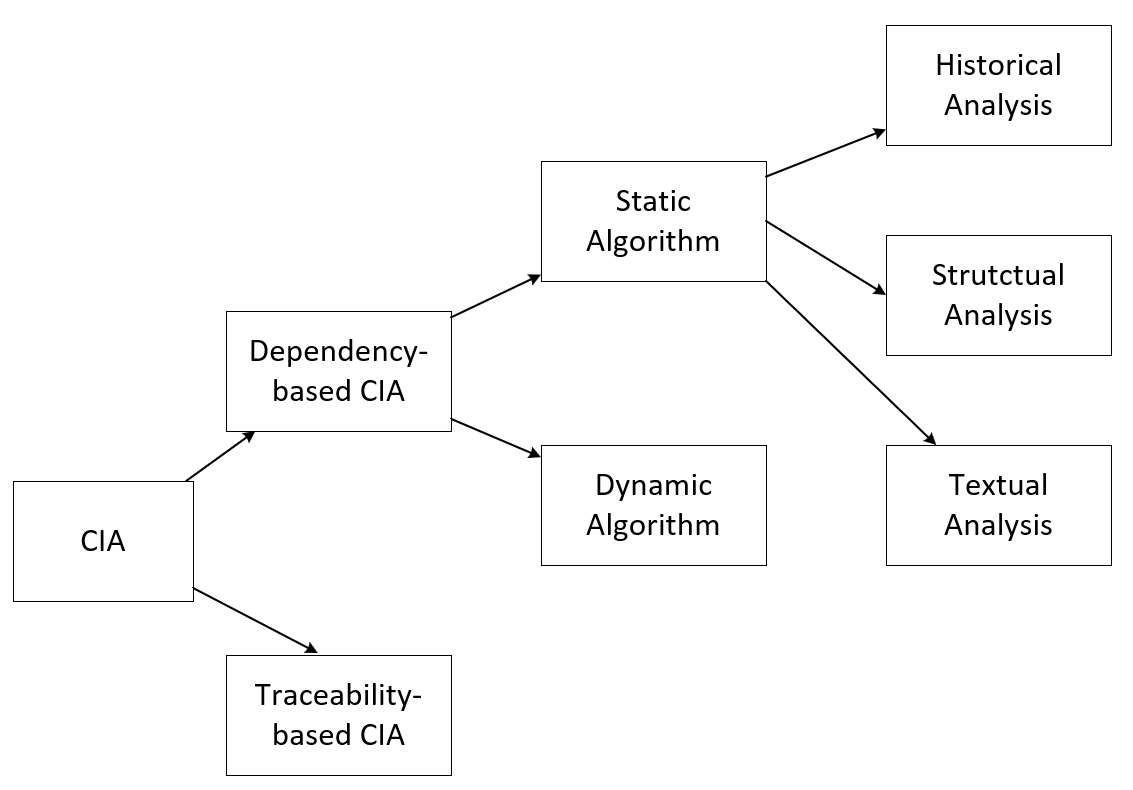
\includegraphics[scale=0.5]{CIA-hierarchy}
	\label{fig:cia-hierarchy}
	\caption{Các phương pháp CIA}
\end{figure}

Trong hơn 30 năm qua, đã có nhiều kỹ thuật CIA được nghiên cứu và đề xuất. Hình \ref{fig:cia-hierarchy} mô tả về các phương pháp CIA hiện nay đã được đề xuất. Một số phương pháp CIA dựa trên phân tích sự truy vết (traceability-based CIA) trong khi một số khác tập trung phân tích các mối quan hệ phụ thuộc (dependency-based CIA) để xác định các ảnh hưởng. Traceability-based CIA sẽ cố gắng truy vết mối liên kết giữa các phần tử trong từng mức trừu tượng với các thành phần tương ứng ở các mức khác (các mức trừu tượng: yêu cầu, tài liệu đặc tả, thiết kế, mã nguồn, ca kiểm thử). Mục tiêu của nó là gắn kết các thể hiện ở mỗi mức trừu tượng khác nhau của các đối tượng phần mềm (ví dụ: tài liệu thiết kế với mã nguồn). Trong khi đó, Depedency-based CIA tập trung xác định các mối quan hệ phụ thuộc của các thành phần trong cùng một mức trừu tượng (ví dụ: mối quan hệ giữa các lớp, phương thức, thuộc tính trong mã nguồn). Depedency-based CIA thường được áp dụng ở mức trừu tượng chi tiết hơn Traceability-based CIA.

Để thực hiện Depedency-based CIA, ta có thể sử dụng hai phương pháp là phân tích tĩnh và động. Phân tích động sẽ yêu cầu thực thi ứng dụng, nó sẽ thu thập các thông tin trước, trong và sau khi chạy để xác định các mối quan hệ phụ thuộc. Phương pháp này mang lại chính xác cao nhưng đòi hỏi sự phức tạp và tốn kém. Bên cạnh đó, các phương pháp phân tích tĩnh dễ thực hiện và ít tốn kém. Chúng tập được thực hiện ngay trên mã nguồn phần mềm. Có thể chia các phương pháp tĩnh này thành ba loại chính: Phân tích dựa trên lịch sử được thực hiện bằng cách khai phá thông tin từ nhiều phiên bản tiến hóa của phần mềm, phương pháp thường cho nhiều kết quả dự đoán nhầm, nhiều phần tử ảnh hưởng dự đoán thật sự không bị ảnh hưởng; Phân tích ngữ nghĩa dựa trên việc trích xuất thông tin từ việc phân tích nội dung comment hoặc các định danh (ví dụ: tên biến, phương thức); Nổi trội nhất trong đó là phân tích cấu trúc, phương pháp này tập trung phân tích tĩnh cấu trúc của chương trình, xác định các mối quan hệ giữa các thành phần và xây dựng đồ thị phụ thuộc.

\section{Quy trình phân tích ảnh hưởng sự thay đổi}
\begin{figure}[h]
	\centering
	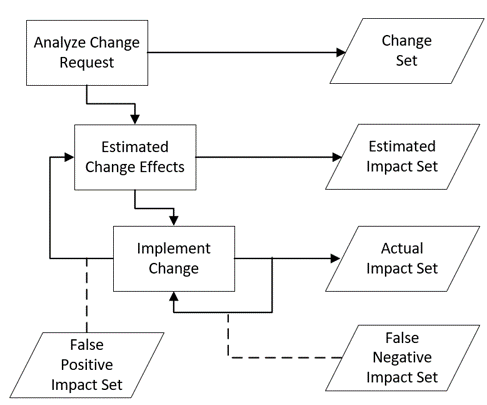
\includegraphics[scale=0.8]{CIA-process}
	\label{fig:cia-process}
	\caption{Quy trình chung CIA}
\end{figure}

Các loại thay đổi trong mã nguồn có thể chia làm hai loại chính là thay đổi cấu trúc và thay đổi lô-gíc. Thay đổi cấu trúc là các thay đổi liên quan đến các thành phần trong mã nguồn. Cụ thể đối với ngôn ngữ Java, thay đổi cấu trúc có thể là thay đổi về phạm vi truy cập, kiểu, tên của một thuộc tính hoặc thay đổi chữ kí của một phương thức. Thay đổi lô-gíc là thay đổi về thuật toán, các câu lệnh. Chúng thường là những thay đổi nằm trong thân phương thức.

Một thay đổi được thực hiện có thể gây ảnh hưởng không mong muốn đến những thành phần mã nguồn khác. Mục tiêu của các kỹ thuật CIA là xác định những thành phần ảnh hưởng. Hình \ref{fig:cia-process} thể hiện toàn bộ quy trình CIA. Phân tích ảnh hưởng sự thay đổi được bắt đầu bằng việc phân tích yêu cầu thay đổi để xác định được tập các thành phần thay đổi (Change Set - CS). Thông qua thuật toán CIA, các thành phần ảnh hưởng sẽ được phán đoán (Estimated Impact Set - EIS). EIS chính là đầu ra cuối cùng của quá trình CIA.

Phương pháp CIA hiệu quả là phương pháp giúp tìm ra được tập ảnh hưởng dự đoán gần nhất với tập ảnh hưởng thực tế khi thực hiện thay đổi (Actual Impact Set - AIS). Khi so sánh giữa EIS và AIS ta, có tập các thành phần ảnh hưởng tiên đoán nhầm (False Negative Impact Set - FNIS) và tập các thành phần ảnh hưởng tiên đoán thiếu (False Positive Impact Set - FPIS). Để đánh giá sự hiệu quả của một phương pháp CIA, người ta dùng hai độ đo là độ chính xác (Precision - P) và Recall - R, được tính theo các công thức \ref{exp:cia-precision} và \ref{exp:cia-recall}. Độ chính xác càng cao, tập FNIS sẽ càng bé, ta ít phải chú ý đến những thành phần không cần thiết. Độ hồi tưởng càng cao, tập FPIS càng bé, giúp ta phát hiện nhiều thành phần bị ảnh hưởng hơn giúp giảm số lỗi tiềm ẩn sau khi áp dụng phương pháp CIA.

\begin{equation}
	Precision = \frac{|EIS \cap AIS|}{EIS}
	\label{exp:cia-precision}
\end{equation}
\\
\begin{equation}
	Recall = \frac{|EIS \cap AIS|}{AIS}
	\label{exp:cia-recall}
\end{equation}

\newpage
\chapter{Phân tích ảnh hưởng sự thay đổi cho các ứng dụng J2EE}
\section{Tiền xử lý mã nguồn ứng dụng J2EE}
\textbf{Định nghĩa:} (\textit{Cây cấu trúc}) Cho mã nguồn ứng dụng J2EE, một cây cấu trúc của mã nguồn này được định nghĩa $T = (N, R)$ với $N = \{n_1, n_2,..., n_k\}$ là tập nút đại diện cho các thành phần trong mã nguồn như thư mục; tệp; lớp, phương thức, thuộc tính (Java); thẻ (XML-based); v,v. $R = \{(n_i, n_j) | n_i,n_j \in N\}$ là tập các cạnh. Mỗi cạnh $(r_i,r_j)$ đại diện cho quan hệ phụ thuộc giữa $n_i$ và $n_j$ có nghĩa là $n_i$ phụ thuộc vào $n_j$.

Các ứng dụng doanh nghiệp J2EE, ngoài sử dụng mã nguồn Java còn nhiều định dạng mã nguồn khác để đảm nhiệm vai trò cho tầng \textit{View} và các thành phần cấu hình ứng dụng như XML, JSP, XHTML, FreeMarker,...Với mỗi một định dạng lại có cấu trúc và cú pháp khác nhau, tuy nhiên ta có thể phân loại thành hai nhóm là mã nguồn Java và mã nguồn XML-based (mã nguồn có cú pháp dựa trên định dạng XML). Bộ tiền xử lý cần biến đổi những mã nguồn này về định dạng chung là cây cấu trúc, các nút trên cây cấu trúc cần chứa những thông tin cần thiết cho việc phân tích phụ thuộc cũng như cây cần được thiết kế để tối ưu cho việc duyệt và tìm kiếm các nút trên cây dễ dàng.

\subsection{Tiền xử lý cho mã nguồn Java và mã nguồn định dạng XML}
Hình \ref{fig:preprocess} thể hiện phương pháp để tiền xử lý mã nguồn ứng dựng J2EE. Hai phương pháp chính được đề xuất để thực hiện tiền xử lý cho mã nguồn Java và mã nguồn XML-based. Một phương pháp duyệt thư mục cũng cần được đề xuất và thực hiện nhằm tìm ra các tệp chứa mã nguồn Java và XML-based trong mã nguồn ứng dụng.

\begin{figure}[h]
	\centering
	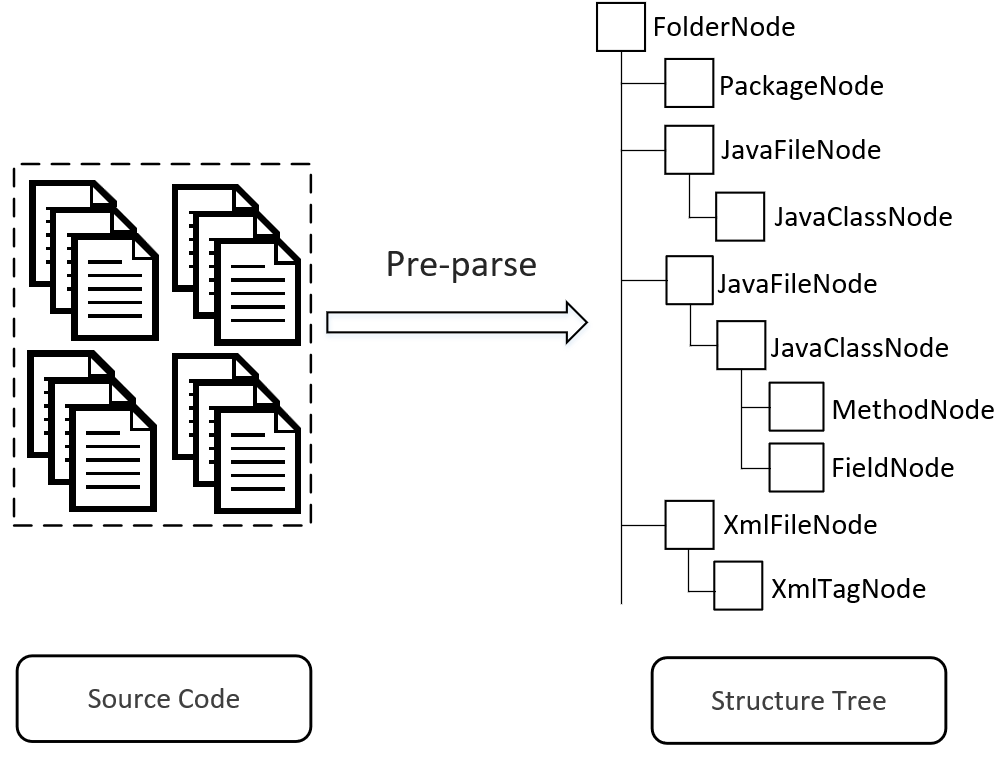
\includegraphics[scale=0.5]{preprocess}
	\label{fig:preprocess}
	\caption{Phương pháp tiền xử lý mã nguồn}
\end{figure}

Đầu tiên, ta thực hiện duyệt toàn bộ cấu trúc các thư mục và tệp trong mã nguồn ứng dụng. Ta có thể sinh được cây cấu trúc cơ bản gồm các nút thư mục và nút tệp. Tiếp theo, ta duyệt tìm tất cả các nút tệp trên cây. Các tệp mã nguồn có phần mở rộng \textit{.java} sẽ được phân tích  để thu thập thông tin và tạo các nút con tương ứng với các thành phần mã nguồn Java đó (lớp, thuộc tính, phương thức). Các thông tin của các thành phần này cũng cần được thu thập (ví dụ: đối với phương thức cần thu thập thông tin về kiểu trả về, mức truy cập, tên phương thức, danh sách các tham số). Hiện nay có một thư viện mã nguồn mở Java có tên Java Development Tools \footnote{https://www.eclipse.org/jdt/} đã hỗ trợ việc phân tích và thu thập thông tin cho các tệp mã nguồn Java. Tuy nhiên đầu ra của thư viện này chứa khá nhiều thông tin không cần thiết. Ta chỉ cần trích xuất những thông tin cần thiết để thêm vào cây cấu trúc. Các tệp mã nguồn có phần mở rộng \textit{.xml, .jsp, .html} sẽ xử lý bởi cùng một phương pháp tiền xử lý cho định dạng mã nguồn dựa trên XML. Kết quả đầu ra sẽ là các nút tương ứng với các thẻ XML có trong tệp. Các nút này cũng cần chứa toàn bộ thông tin của thẻ đấy, bao gồm các thuộc tính và nội dung của thẻ.

\subsection{Định danh các nút trên cây cấu trúc}
Cây cấu trúc là dữ liệu được sử dụng xuyên suốt trong các quá trình phân tích. Sẽ có rất nhiều hoạt động phân tích cần đến việc tìm kiếm và truy xuất dữ liệu của các nút trên cây. Vì thế việc định danh cho các nút trên cây là một việc rất quan trọng. Phương pháp đề xuất là định danh bằng đường dẫn tuyệt đối của nút. Đường dẫn tuyệt đối của mỗi nút trên cây sẽ được tạo thành bởi tên lần lượt của các nút cha và tên của nó, ngăn cách bởi kí tự gạch chéo (\texttt{/}). Với hầu hết các nút đại diện trong thành phần mã nguồn sẽ có đường dẫn tuyệt đối duy nhất, ta có thể thực hiện \textit{Indexing} các nút trên cây phục vụ cho việc tìm kiếm nhanh. Tuy nhiên, trong một số trường hợp, dùng tên các nút để tạo thành đường dẫn tuyệt đối sẽ có thể cho cùng một kết quả đối với nhiều hơn một nút.

\begin{lstlisting}[language=Java,
caption={Ví dụ chồng hàm trong Java},label={code:java-overloading}]
package vn.sample.manager.BookManager;
import vn.sample.model.Boook;
import vn.sample.model.Author;
public class BookManager {
	//...	
	public void addBook(Book newBook) {
		//...
	}
	public void addBook(String bookName, Author author) {
		//...
	}
}
\end{lstlisting}

Ví dụ như ở Mã nguồn \ref{code:java-overloading} thể hiện sự chồng hàm của phương thức \texttt{addBook()}. Nếu chỉ sử dụng tên của phương thức thì ta sẽ không định danh cho các các nút tương ứng với hai phương thức này được. Do vậy ta cần sử dụng cả thông tin về các tham số của chúng để tạo đường dẫn tuyệt đối. Bao gồm cả tên, kiểu có tên xác định hoàn toàn (Fully qualified name) và thứ tự của các tham số này trong phần khai báo phương thức. Kết quả ta được hai đường dẫn tuyệt đối có thể đại diện cho sự riêng biệt của các nút phương thức Java này.

\begin{verbatim}
vn/sample/manager/BookManager.java/BookManager/
addBook(vn.sample.model.Book_newBook)

vn/sample/manager/BookManager.java/BookManager/
addBook(java.lang.String_bookName,java.lang.String_author)
\end{verbatim}

Hoặc đối với mã nguồn dựa trên định dạng XML như ở Mã nguồn \ref{code:html-example}, nếu dùng tên thẻ để làm đường dẫn tuyệt đối thì hai phần tử \texttt{h1} sẽ có chung giá trị là \texttt{web/hello.html/html/body/h1}. Để định danh cho hai phần này, ta sẽ dùng thêm các thuộc tích đặc biệt là tọa độ thẻ mở của chúng trong mã nguồn. Ví dụ với phần \texttt{h1} đầu tiên, sẽ có tọa độ số dòng là 3, số cột là 12 cho nên đường dẫn tuyệt đối của nó sẽ là \texttt{web/hello.html/html/body/h1:3:12}. Đường dẫn mới này sẽ giúp phân biệt phần tử này với phần liền kề với đường dẫn \texttt{web/hello.html/html/body/h1:4:12}. Thật may mắn nền tảng Java cung cấp sẵn một thư viện giúp chúng ta phân tích các tệp có định dạng XML và lấy được tọa độ của các phần tử này. SAXParser sẽ giúp ta tiết kiệm công sức rất nhiều trong việc tiền xử lý phần mã nguồn này.

\begin{lstlisting}[language=XML,
caption={Ví dụ mã nguồn HTML},label={code:html-example}]
<html>
	<body>
		<h1>Hello!</h1>
		<h1>I am writing this line with Latex.</h1>
	</body>
</html>
\end{lstlisting}

\subsection{Xác định tên xác định hoàn toàn cho kiểu Java}
Với yêu cầu tham số có kiểu xác định hoàn toàn phụ vụ cho việc định danh cho phương thức Java, ta cần phải thực hiện xử lý qua một số bước như sơ đồ khối ở Hình \ref{fig:fqn-type}.

\begin{figure}[h]
	\centering
	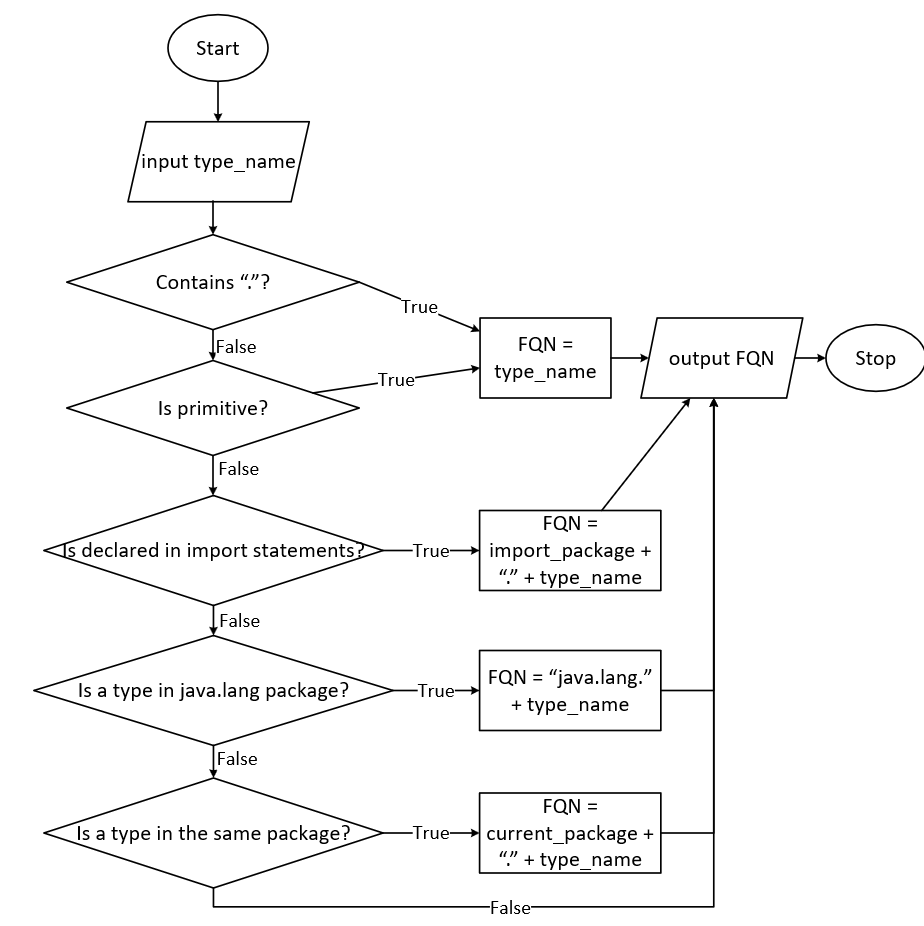
\includegraphics[scale=0.6]{fqn-type}
	\label{fig:fqn-type}
	\caption{Xác định tên xác định hoàn toàn cho kiểu Java}
\end{figure}

\section{Phân tích phụ thuộc Struts}
\subsection{Giới thiệu mô hình kiến trúc Struts}
Apache Struts (trước đây được gọi là Struts2 để phân biệt với Struts1) là một trong những framework được ưa chuộng nhất để phát triển các ứng dụng web J2EE. Tương tự Spring MVC, Struts tuân theo mô hình xử lý MVC mà bản thân nó chứa đủ các thành phần giúp lập trình viên định nghĩa rõ ràng các thành phần Model, View và Controller.

\begin{figure}[h]
	\centering
	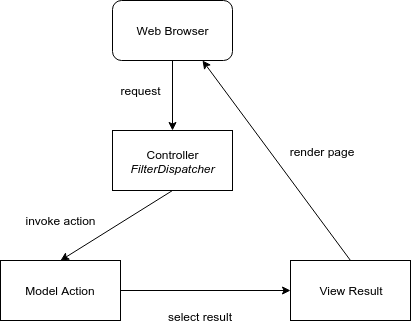
\includegraphics[scale=0.8]{struts-architecture}
	\label{fig:struts-architecture}
	\caption{Mô hình thiết kế của ứng dụng Struts}
\end{figure}

Hình \ref{fig:struts-architecture} thể hiện mô hình thiết kế của một ứng dụng Struts. Các thành phần chính của nó được thiết kế tương ứng với các phần trong mô hình MVC chung.

\textbf{Model:} là các lớp Java định nghĩa các đối tượng để chứa dữ liệu (POJO). Chúng chỉ đơn thuần có phương thức getter/setter tương ứng với các thuộc tính.

\textbf{View:} là các tệp JSP, dùng để hiển thị dữ liệu tới người dùng. Việc lấy dữ liệu từ Model để hiển thị lên View được thực hiện nhờ một thành phần trong Struts có tên là OGNL (Object-graph Navigation Language).

\textbf{Controller:} là phần xử lý lô-gíc, trong Struts được gọi là Action. Mỗi Action sẽ là một lớp Java, thường kế thừa từ lớp \textit{ActionSupport} của Struts. Trong lớp Action này có chứa tham chiếu đến lớp Java của phần Model, từ đó có thể dễ dàng truy cập dữ liệu từ phần Model. Các phương thức bên trong lớp Action sẽ thực hiện truy xuất và xử lý dữ liệu từ lớp Model. Sau khi thực hiện xử lý xong, phương này có thể cập nhật lại dữ liệu và chuyển hướng đến một View tương ứng để hiển thị kết quả tới người dùng.

\subsection{Làm mịn cây cấu trúc}

\begin{figure}[h]
	\centering
	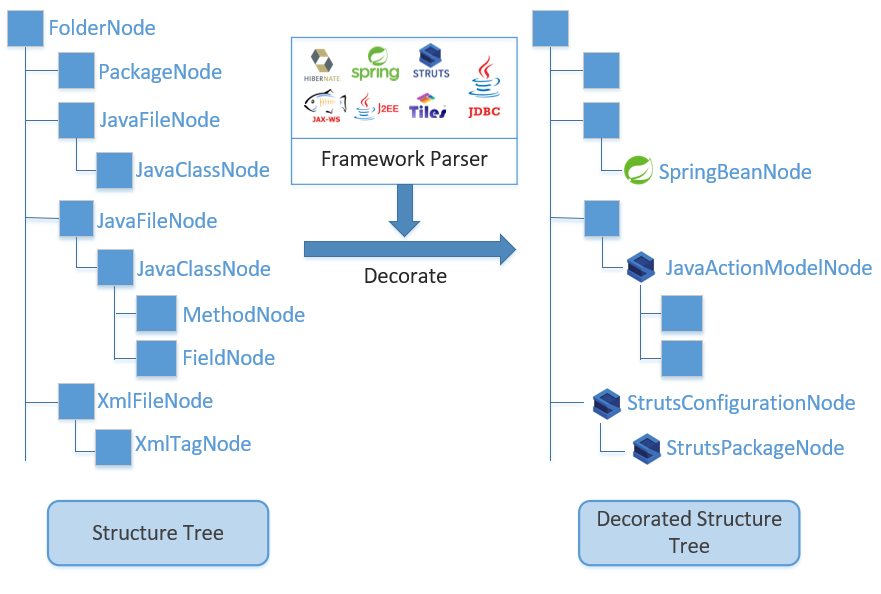
\includegraphics[scale=0.6]{lam-min}
	\label{fig:lam-min}
	\caption{Làm mịn cây cấu trúc}
\end{figure}

Các nút trên cây sau khi được tiền xử lý mới chỉ mang thông tin cơ bản đặc trưng cho ngôn ngữ được tiền xử lý. Tuy nhiên, công việc phân tích phụ thuộc cần nhiều thông tin hơn nữa để xác định các quan hệ phụ thuộc. Đối với một framework, sẽ có một phương pháp riêng để trích xuất thông tin đặc trưng này. Bước thực hiện này được gọi là làm mịn cây câu trúc. Đối với Struts cũng vậy, ta cần làm mịn các nút thành phần Java và XML thành các nút đặc trưng của Struts như \textit{JavaActionModelNode, StrutsConfigurationNode, StrutsPackageNode} được minh họa ở Hình \ref{fig:lam-min}.

Với yêu cầu thực hiện chuyển đổi từ một nút ban đầu trên cây sang một nút hoàn toàn mới nhưng vẫn giữ được các thuộc tính và phương thức của nút cũ, ta dùng mẫu thiết kế \textit{Decorator}. Ví dụ cho việc chuyển đổi từ nút \textit{XmlFileNode} sang nút \textit{StrutsConfiguration} được minh họa ở Mã nguồn \ref{code:decorator-dp}.

\begin{lstlisting}[language=Java,
caption={Ví dụ sử dụng mẫu thiết kế Decorator},label={code:decorator-dp}]
public class StrutsConfigurationNode extends XmlFileNode {
	protected XmlFileNode xmlFileNode;
	
	protected List<StrutsPackage> strutsPackages;
	protected Lits<StrutsConfigurationNode> includedNodes;
	// constructor
	@Override
	public String getDocument() {
		return xmlFileNode.getDocument();
	}
	//...
}
\end{lstlisting}

Lớp \textit{StrutsConfigurationNode} được thiết kế kế thừa đồng thời chứa một thực thể \textit{XmlFileNode}, nó cho phép tái sử dụng lại thông tin nút \textit{XmlFileNode} trước đó (ví dụ: phương thức \textit{getDocument()}). Ngoài ra nó cũng phép định nghĩa thêm các thuộc tính và phương thức mới như \textit{strutsPackages}, \textit{includedNodes}.

\begin{figure}[h]
	\centering
	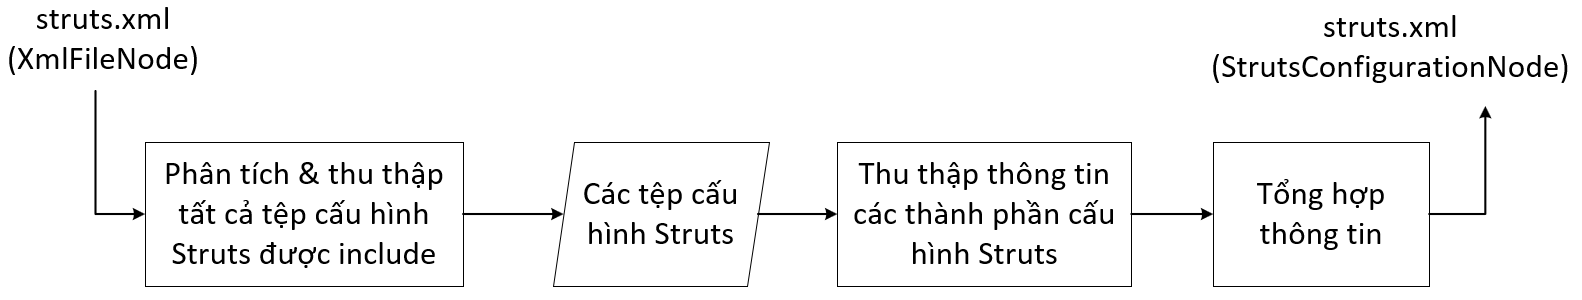
\includegraphics[scale=0.5]{lam-min-process}
	\label{fig:lam-min-process}
	\caption{Quá trình làm mịn các nút thành phần Struts}
\end{figure}

Hình \ref{fig:lam-min-process} biểu diễn quá trình làm mịn cho các thành phần Struts từ khi là một nút \textit{XmlFileNode} đến khi trở thành nút \textit{StrutsConfigurationNode}. \textit{struts.xml} là tệp cấu hình cho framework Struts trong một ứng dụng J2EE có sử dụng Struts. Để tránh sự phức tạp cho tệp này và để dễ quản lý các thành phần cấu hình theo từng chức năng, Struts cho phép chúng ta khai báo nhiều tệp cấu hình tuy chúng cần được khai báo trong \textit{struts.xml} thì framework mới sử dụng các cấu hình được định nghĩa trong chúng. Muốn thu thập tất cả thông tin cấu hình, ta cần thu thập và phân tích tất cả tệp cấu hình này. Sau đấy, ta sẽ thu thập toàn bộ thông tin về các thành phần cấu hình của Struts như \textit{Result Type, Interceptor, Result, Action} và \textit{Package}. Do các thông tin cấu hình được chia nhỏ ra ở nhiều tệp, nên có thể một thông tin cấu hình có thể được định nghĩa ở nhiều tệp (ví dụ: một \textit{Package} có thể được định nghĩa ở nhiều tệp). Những thông tin này cần được tổng hợp lại và loại bỏ những trùng lặp hoặc ghi đè ở bước tổng hợp thông tin. Cuối quá trình làm mịn này, ta sẽ thu được một nút \textit{StrutsConfiguration}, từ nó ta có thể có mọi thông tin cấu hình Struts của ứng dụng.

\subsection{Xác định quan hệ phụ thuộc các thành phần Struts}
Sau khi đã thực hiện làm mịn và thu được nút chứa toàn bộ thông tin cấu hình, việc xác các quan hệ phụ thuộc Struts (giữa mã nguồn ở ba phần Model, View và Controller) sẽ dựa trên duyệt các thành phần cấu hình. Quá trình xác định phụ thuộc này được biểu diễn ở Hình \ref{fig:struts-analyzer}.

\begin{figure}[h]
	\centering
	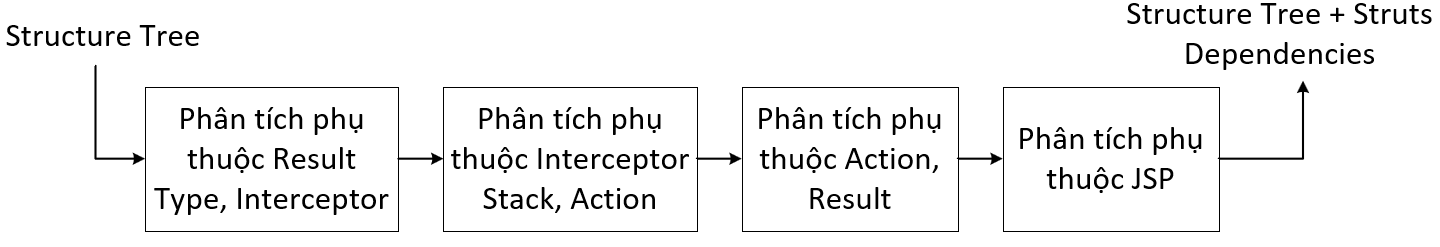
\includegraphics[scale=0.55]{struts-analyzer}
	\label{fig:struts-analyzer}
	\caption{Xác định các quan hệ phụ thuộc Struts}
\end{figure}

Đầu tiên, thực hiện xác định quan hệ phụ thuộc cho các thành phần \textit{Result Type} và \textit{Interceptor} bởi chúng chỉ có duy nhất một mối quan hệ phụ thuộc với Model xử lý nghiệp vụ phía sau. Tiếp theo, thực hiện phân tích cho các thành phần \textit{Interceptor Stack}, \textit{Result} bởi chúng sử dụng các thành phần \textit{Result Type, Interceptor}. Ngoài ra \textit{Result} còn có mối quan hệ phụ thuộc với các tệp \textit{.jsp} ở phần View. Trong một số trường hợp khác, ứng dụng có thể sử dụng plugin Tiles \footnote{https://tiles.apache.org} nhằm thiết kế layout cho các tệp \textit{.jsp}. Lúc đấy, ta không thể xác định quan hệ phụ thuộc trực tiếp từ \textit{Result} sang phần View mà phải thông qua các thành phần cấu hình của Tiles. Tiếp đến, các \textit{Action} được phân tích bởi nó sử dụng \textit{Interceptor Stack, Interceptor} và là thành phần cha của \textit{Result}. Nó cũng có mối quan phụ thuộc đến thành phần mã nguồn Java để xử lý phía sau. Sau khi đã xác định được toàn bộ các quan hệ phụ thuộc của phần Controller (các thành phần cấu hình) tới phần Model và View, ta sẽ sử dụng chúng để phân tích phụ thuộc cho phần View. Cụ thể là truy vết theo các quan hệ phụ thuộc của một bộ Controller - Model - View để xác định các quan hệ sử dụng dữ liệu từ View đến Model tương ứng của nó.

\subsection{Ví dụ minh họa}

\begin{figure}[h]
	\centering
	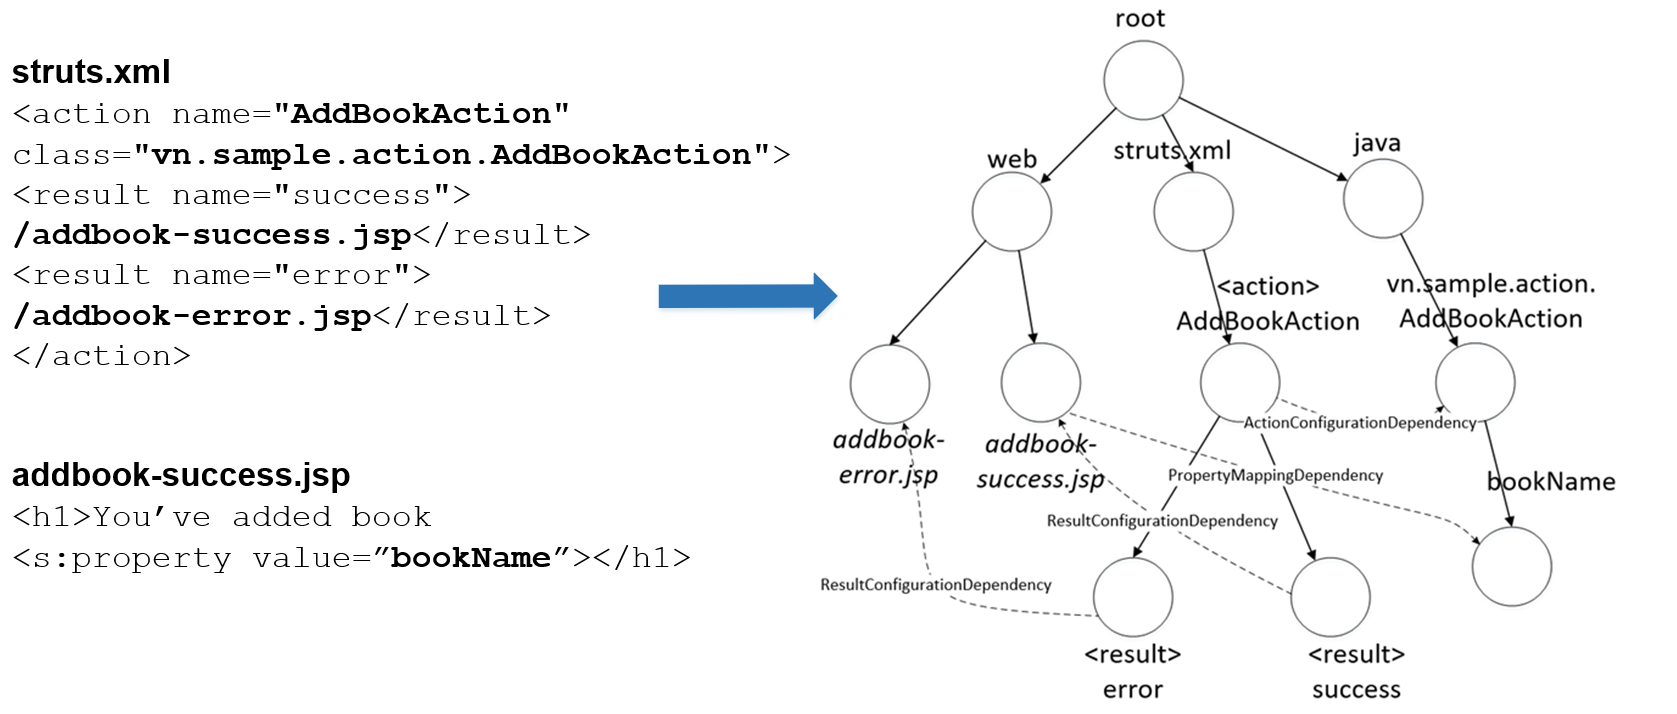
\includegraphics[scale=0.53]{struts-analyzer-sample}
	\label{fig:struts-analyzer-sample}
	\caption{Ví dụ minh họa xác định các quan hệ phụ thuộc Struts}
\end{figure}

Để hiểu rõ về quá trình phân tích và xác định phụ thuộc cho các thành phần Struts, một ví dụ minh họa đơn giản sẽ được trình bày như ở Hình \ref{fig:struts-analyzer-sample}.

Đầu tiên, đối với thành phần cấu hình \textit{Action} có tên \textbf{AddBookAction}, ta thu được một quan hệ phụ thuộc từ nó đến lớp Java \textbf{vn.sample.action.AddBookAction}. Tiếp theo đó, tiếp tục phân tích cho hai thành phần cấu hình \textit{Result} có tên là \textbf{success} và \textbf{error} thu được hai phụ thuộc từ chúng ra phần View là hai tệp \textbf{/addbook-success.jsp} và \textbf{/addbook-error.jsp}.

Lúc này, ta đã thu thập được toàn bộ các quan hệ phụ thuộc cấu hình của Struts. Khi phân tích tệp \textbf{/addbook-success.jsp}, ta thấy nó có sử dụng một thuộc tính có tên \textbf{bookName}. Câu hỏi đặt ra là thuộc tính được sử dụng này được định nghĩa ở thành phần nào. Ta sẽ phải truy vết phụ thuộc từ chính tệp \textit{.jsp} này xem nó được sử dụng bởi \textit{Action} nào, từ đó tìm ra phần mã nguồn Model tương ứng để xác định quan hệ phụ thuộc sử dụng thuộc tính của Model. Như ở ví dụ trên, ta có thể thấy \textbf{/addbook-success.jsp} được sử dụng bởi \textbf{AddBookAction}, có Model tương ứng là \textbf{vn.sample.action.AddBookAction}. Từ đấy ta xác định quan hệ phụ thuộc sử dụng dữ liệu từ thẻ \textbf{<s:property>} để thuộc tính \textbf{bookName} của lớp Java \textbf{vn.sample.action.AddBookAction}.

\section{Phương pháp phân tích ảnh hưởng sự thay đổi WAVE-CIA}

\begin{figure}[h]
	\centering
	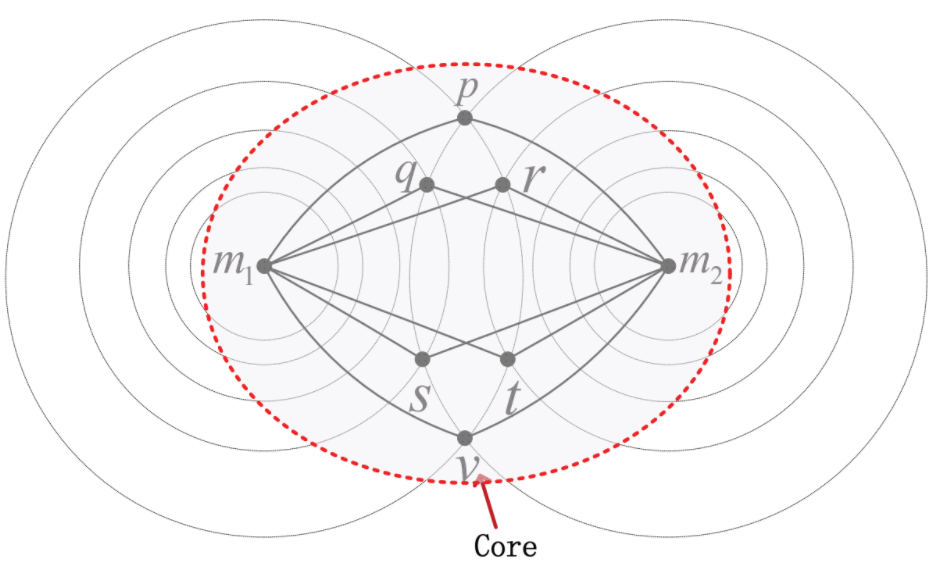
\includegraphics[scale=0.45]{wave-cia-phenomenon}
	\label{wave-cia-phenomenon}
	\caption{Hiện tượng lan truyền sóng nước trên đồ thị gọi}
\end{figure}

Trong việc xây dựng công cụ này, WAVE-CIA được sử dụng làm phương pháp phân tích ảnh hưởng sự thay đổi. WAVE-CIA là một phương pháp phân tích tĩnh trực tiếp trên mã nguồn ứng dụng, sử dụng một bản biểu diễn chương trình dưới dạng đồ thị gọi (Call Graph - CG) tĩnh. Ý tưởng của phương pháp này dựa trên sự mô phỏng hiện tượng lan truyền sóng nước, được mô tả như Hình \ref{wave-cia-phenomenon}. Hầu hết các phương pháp CIA đưa ra dự đoán tập ảnh hưởng dựa trên từng thành phần riêng lẻ của tập thay đổi chứ không xem xét mối quan hệ giữa chúng. Trong khi đó, nhiều thay đổi có thể được thực hiện cùng lúc để đáp ứng một yêu cầu thay đổi nào đó. WAVE-CIA dựa trên nguyên tắc này, và nó có thể dự đoán tập ảnh hưởng tốt hơn với tập thay đổi gồm nhiều phần tử.

Để thực hiện phương pháp này, một đồ thị gọi cần được xây dựng đầu tiên. Sau đó, những phần tử tập cốt lõi sẽ được tìm ra, tập ảnh hưởng cuối cùng sẽ được tính toán dựa vào tập cốt lõi.

\subsection{Xây dựng đồ thị gọi}
Đồ thị gọi là một đồ thị có hướng $G = (V, E)$. $V$ là tập các đỉnh tương ứng với các nút trong cây cấu trúc (lớp, phương thức, thuộc tính Java; phần tử XML; tệp JSP, HTML), và $E \subseteq V \times V$ là tập các cạnh biểu diễn cho các mối quan hệ phụ thuộc giữa các nút này.

Để xây dựng được đồ thị gọi cho phương pháp CIA, ta chỉ cần chuyển đổi từ cây cấu trúc. Các bước để thực hiện được trình bày ở Thuật toán \ref{algo:build-call-graph}.

\begin{thuattoan}
	\label{algo:build-call-graph}
	\caption{Xây dựng đồ thị gọi từ cây cấu trúc}
	\SetKwInOut{Input}{Input}
	\SetKwInOut{Output}{Output}
	\SetKwInOut{Use}{Use}
	\Input{$T = (N, R)$ là cây cấu trúc của ứng dụng}
	\Output{$G = (V, E)$ là đồ thị gọi của ứng dụng}
	\Use{$getCallees(n)$ là các nút được gọi hoặc sử dụng bởi $n$}
	V = $\emptyset$, E = $\emptyset$\;
	\ForEach{$n \in N$}{
		$V = V \cup \{n\}$\; 
		\ForEach{$ne \in getCallees(n)$} {$E = E \cup (n, ne)$\;}
	} 
	\Return V\;
\end{thuattoan}

\subsection{Xác định tập cốt lõi}
Như đã nói ở trên, hầu hết các phương pháp CIA hiện nay tính toán tập ảnh hưởng mà không quan tâm đến mối quan hệ của các phần tử trong tập thay đổi. Trong thực tế, luôn có mối quan hệ giữa các phần tử trong tập thay đổi. Chúng ta sẽ sử dụng hiện tượng này trong việc ước tính tập ảnh hưởng. Đầu tiên ta cần tìm tập cốt lõi, nó là tập gồm các thành phần thường bị ảnh hưởng bởi nhiều phần tử trong tập thay đổi nhất. Việc tính toán tập cốt lõi được thực hiện bằng việc khai thác thông tin từ đồ thị gọi, các bước thực hiện như Thuật toán \ref{algo:cal-core-set}.

\begin{thuattoan}
	\label{algo:cal-core-set}
	\caption{Xác định tập cốt lõi}
	\SetKwInOut{Input}{Input}
	\SetKwInOut{Output}{Output}
	\SetKwInOut{Use}{Use}
	\Input{
		$G = (V, E)$ là đồ thị gọi của ứng dụng\\
		$CS$ gồm những phần tử của tệp thay đổi\\
		$depth$ là độ sâu tìm kiếm
	}
	\Output{$Core$ là tập cốt lõi}
	\Use{$getNeighborSet(m, depth)$ là tập các đỉnh có quan hệ với đỉnh $m$ với khoảng cách $depth$}
	
	$tempSet = \emptyset$\;
	\ForEach{$v \in V$}{
		$neighborSet = getNeighborSet(m, depth)$\;
		$neighborCSSet = neighborSet \cap CS$\;
		\If{$|neighborSet| > 1$} {$tempSet = tempSet \cup \{m\}$}
	}
	$Core = CS \cup tempSet$\;
	\Return $Core$\;
\end{thuattoan}

Các phần tử trong tập cốt lõi được định nghĩa là các đỉnh \textit{láng giềng} với nhiều hơn một phần tử trong tập thay đổi. \textit{Láng giềng} tức là có quan hệ phụ thuộc giữa hai đỉnh trên đồ thị gọi nhỏ hơn một khoảng cách $depth$ cho trước. Khoảng cách $depth$ sẽ thay đổi với từng bài toán để cân bằng giữa độ chính xác và độ hồi tưởng của phương pháp để phù với từng loại yêu cầu cụ thể (ví dụ: cần độ chính xác cao thay vì quan tâm đến độ hồi tưởng cao).

\subsection{Tính toán tập ảnh hưởng}
Mặc dù tập cốt lõi có thể cho kết quả có độ chính xác tốt nhờ vào điều chỉnh $depth$, tuy vẫn có những phần tử bị dự đoán ảnh hưởng thiếu (thực tế phần tử đó bị ảnh hưởng nhưng không xuất hiện trong tập cốt lõi). Do vậy ta cần tính toán để tìm thêm các phần tử còn sót này, ta sẽ mở rộng tập cốt lõi để xây dựng tập ảnh hưởng cuối cùng (Final Impact Set - FIS) nhằm tăng độ hồi tưởng cho phương pháp. Phương pháp tính toán FIS được thể hiện như Thuật toán \ref{algo:cal-fis}.

\begin{thuattoan}
	\label{algo:cal-fis}
	\caption{Tính toán tập ảnh hưởng}
	\SetKwInOut{Input}{Input}
	\SetKwInOut{Output}{Output}
	\SetKwInOut{Use}{Use}
	\Input{
		$G = (V, E)$ là đồ thị gọi của ứng dụng\\
		$Core$ là tập cốt lõi\\
	}
	\Output{$FIS$ là tập ảnh hưởng}
	\Use{$getCallerSet(m, depth)$ là tập các đỉnh gọi hoặc sử dụng $m$ trong khoảng cách $depth$\\
		$getCalleeSet(m, depth)$ là tập các đỉnh được gọi hoặc sử dụng bởi $m$ trong khoảng cách $depth$\\}
	
	
	$FIS = Core$\;
	\While{$FIS$ có số lượng phần tử không ổn định} {
		\ForEach{$v \in V$}{
			\If{$m \notin FIS$}{
				$callerSet = getCallerSet(v)$\;
				$calleeSet = getCalleeSet(v)$\;
				\If{$FIS \cap callerSet \neq \emptyset \wedge FIS \cap calleeSet \neq \emptyset$}{
					$FIS = FIS \cup \{v\}$
				}
			}
		}
	}
	
	\Return $FIS$\;
\end{thuattoan}

Một phần tử $v$ sẽ được thêm vào tập ảnh hưởng nếu $v$ thỏa mãn điều kiện khi $v$ được gọi hoặc sử dụng bởi $v_1$ và $v_2$, hoặc ngượi lại $v_1$ và $v_2$ gọi hoặc sử dụng $v$; trong khi $v_1$ và $v_2$ là hai phần tử thuộc tập cốt lõi. Sau khi duyệt tất cả các phần tử, tập ảnh hưởng có thể được sử dụng tiếp như tập cốt lõi để tiếp tục mở rộng tập ảnh hưởng nếu nó chưa đủ tốt để tăng độ phủ cho phương pháp. Thuật toán có thể dừng lại khi kích thước tập ảnh hưởng đạt mức ổn định.

\chapter{Quản lý các phiên bản}
Các nhà bảo trì phần mềm cần phải hiểu về ứng dụng phần mềm trước khi thực hiện các sửa đổi trên nó. Mặc dù mã nguồn hệ thống thường được xem xét (review) cẩn thận, tuy nhiên chỉ xem xét cho mã nguồn ở phiên bản hiện tại là không đủ để hiểu rõ sự tiến hóa của nó. Các nhà bảo trì cũng nên hiểu được mã nguồn đã được thay đổi như thế nào trước đó.

Quản lý phiên bản là công việc lưu trữ các thay đổi của ứng dụng phần mềm theo thời gian, nó có thể giúp ta theo dõi các thay đổi qua thời phát triển, bảo trì và hoàn toàn có thể khôi phục lại một phiên bản xác định nào đó sau này. Một số hệ thống quản lý phiên bản phổ biến hiện nay như Git \footnote{https://git-scm.com} hay SVN  \footnote{https://subversion.apache.org} tập trung lưu trữ các thay đổi ở mức các dòng mã nguồn. Các hệ thống này có thể trích xuất thông tin về sự khác nhau giữa các lần sửa đổi của một tệp mã nguồn được lưu trữ. Một tập hợp các thông tin này được xem như là lịch sử thay đổi của tệp mã nguồn đấy.

Tuy nhiên, trong thực tế có một vài bất lợi cho các nhà bảo trì khi sử dụng các hệ thống này để theo dõi lịch sử thay đổi của ứng dụng phần mềm. Ở mỗi lần cam kết (commit - xác nhận lưu trữ thay đổi), lập trình viên thường sửa đổi rất nhiều thứ xen kẽ nhau chứ không chỉ thực hiện một thay đổi. Các công cụ phát hiện ở mức dòng mã nguồn khó tách rời những thay đổi này ra và phát hiện riêng rẽ từng thay đổi trong một lần cam kết đấy. Nếu các nhà bảo trì phải thực hiện công việc này bằng tay, nó sẽ tốn rất nhiều thời gian và chi phí.

Để giải quyết vấn đề nhiều thay đổi xuất hiện xen kẽ trong cùng một lần cam kết. Một hướng tiếp cận để phát hiện thay đổi mới được để xuất. Cơ chế này sẽ phát hiện thay đổi trên một dạng dữ liệu trừu tượng là cây cấu trúc của các phiên bản ứng dụng chứ không phải những dòng mã nguồn. Trong các chương trình hướng đối tượng như J2EE, các lớp, phương thức, thuộc tính sẽ thích hợp làm đơn vị cho các thay đổi. Việc sử dụng cây cấu trúc làm dữ liệu để thực hiện phát hiện thay đổi so với dòng mã giúp trừu tượng hóa các thay đổi, giảm lượng thông tin cần xử lý cho người bảo trì nhưng vẫn cung cấp đủ thông tin để họ có thể hiểu sự tiến hóa của ứng dụng. Ngoài việc cung cấp đầu vào cho việc lưu trữ thay đổi, cơ chế so sánh này còn giúp ích trong việc tự động thực hiện phân tích ảnh hưởng sự thay đổi. Các thành phần mã nguồn thay đổi được thu thập từ bộ so sánh được sử dụng làm tập thay đổi cho thuật toán CIA.

\section{Phát hiện thay đổi cho mã nguồn Java}
Các thành phần mã nguồn Java có thể chia làm ba loại chính gồm lớp, phương thức và thuộc tính. Có rất nhiều loại thay đổi đối với những thành phần mã nguồn này, ví dụ như mở rộng mức truy cập từ \textit{private} thành \textit{public}, thay đổi lớp cha đối với lớp hoặc thay đổi tham số đối với phương thức, v.v. Tất cả các loại thay đổi cho Java được liệt kê ở các Bảng \ref{tbl:field-ct} và Bảng \ref{tbl:class-method-changes}.


\begin{table}[h]
	\centering
	\caption{Các loại thay đổi của thuộc tính Java}
	\label{tbl:field-ct}
	\begin{tabular}{|l|l|}
		\hline
		\textbf{Kí hiệu} & \textbf{Ý nghĩa}                                        \\ \hline
		AF               & Thêm thuộc tính mới                                            \\ \hline
		DF               & Xóa thuộc tính                                                 \\
		\hline
		CNF               & Đổi tên thuộc tính                                                 \\
		\hline
		IAF              & Mở rộng mức truy cập của thuộc tính                            \\ \hline
		DAF              & Thu hẹp mức truy cập của thuộc tính                            \\ \hline
		AFF              & Thêm từ khóa \textit{final} cho thuộc tính    \\ \hline
		DFF              & Xóa từ khóa \textit{final} của thuộc tính     \\ \hline
		ASF              & Thêm từ khóa \textit{static} cho thuộc tính   \\ \hline
		DSF              & Xóa từ khóa \textit{static} của thuộc tính    \\ \hline
		CSF              & Thay đổi kiểu của thuộc tính    \\ \hline
	\end{tabular}
\end{table}

\begin{table}[h]
	\centering
	\caption{Các loại thay đổi của lớp và phương thức Java}
	\label{tbl:class-method-changes}
	\begin{tabular}{|l|p{6cm}|l|p{6cm}|}
		\hline
		\textbf{Kí hiệu} & \textbf{Ý nghĩa}                                        & \textbf{Kí hiệu} & \textbf{Ý nghĩa}                                                \\ \hline
		\multicolumn{2}{|l|}{\textit{Các loại thay đổi của lớp}}                   & \multicolumn{2}{l|}{\textit{Các loại thay đổi của phương thức}}                    \\ \hline
		AC               & Thêm lớp mới                                            & AM               & Thêm phương thức mới                                            \\ \hline
		DC               & Xóa lớp                                                 & DM               & Xóa phương thức                                                 \\ \hline
		CNC              & Đổi tên lớp                                             & CNM              & Đổi tên phương thức                                             \\ \hline
		IAC              & Mở rộng mức truy cập của lớp                            & IAM              & Mở rộng mức truy cập của phương thức                            \\ \hline
		DAC              & Thu hẹp mức truy cập của lớp                            & DAM              & Thu hẹp mức truy cập của phương thức                            \\ \hline
		AFC              & Thêm từ khóa \textit{final} cho lớp    & AFM              & Thêm từ khóa \textit{final} cho phương thức    \\ \hline
		DFC              & Xóa từ khóa \textit{final} của lớp     & DFM              & Xóa từ khóa \textit{final} của phương thức     \\ \hline
		ASC              & Thêm từ khóa \textit{static} cho lớp   & ASM              & Thêm từ khóa \textit{static} cho phương thức   \\ \hline
		DSC              & Xóa từ khóa \textit{static} của lớp    & DSM              & Xóa từ khóa \textit{static} của phương thức    \\ \hline
		AAbC             & Thêm từ khóa \textit{abstract} cho lớp & AAbM             & Thêm từ khóa \textit{abstract} cho phương thức \\ \hline
		DAbC             & Xóa từ khóa \textit{abstract} của lớp  & DAbM             & Xóa từ khóa \textit{abstract} của phương thức  \\ \hline
		APC              & Thêm lớp cha                                            & CM               & Thay đổi nội dung thân phương thức                              \\ \hline
		DPC              & Xóa lớp cha                                             & CRM              & Thay đổi kiểu trả về của phương thức                            \\ \hline
		CPC              & Thay đổi lớp cha                                        & CPM              & Thay đổi danh sách tham số của phương thức                      \\ \hline
	\end{tabular}
\end{table}

\begin{thuattoan}
	\label{algo:class-change}
	\caption{$ClassChange(F_{t1}, F_{t2})$}
	\SetKwInOut{Input}{Input}
	\SetKwInOut{Output}{Output}
	\Input{$F_{t1}, F_{t2}$ lần lượt đại diện cho các nút của tệp chứa thay đổi ở phiên bản $t1$ và $t2$}
	\Output{$CS$ là danh sách các thay đổi}
	
	$C_{t1}$ = tất cả lớp trong $F_{t1}$\;
	$C_{t2}$ = tất cả lớp trong $F_{t2}$\;
	CS = $\emptyset$\;
	\ForEach{$c_1 \in C_{t1}, c_2 \in C_{t2}$}{
		\If{$c_1.name = c_2.name$}{
			$CS = CS \cup compareFinalModifier(c_1, c_2)$\;
			$CS = CS \cup compareVisibilityModifier(c_1, c_2)$\;
			$CS = CS \cup compareStaticModifier(c_1, c_2)$\;
			$CS = CS \cup compareAbstractModifier(c_1, c_2)$\;
			\If{$c_1.parent = null \wedge c_2.parent \neq null$} {
				$CS = CS \cup (c_1, APC)$\;
			}\ElseIf{$c_1.parent \neq null \wedge c_2.parent = null$}{
				$CS = CS \cup (c_1, DPC)$\;
			}\ElseIf{$c_1.parent \neq null \wedge c_1.parent \neq c_2.parent$}{
				$CS = CS \cup (c_1, CPC)$\;
			}
			$CS = CS \cup FieldChange(c_1, c_2)$\;
			$CS = CS \cup MethodChange(c_1, c_2)$\;
			$C_{t1} = C_{t1} \setminus \{c_1\}$\;
			$C_{t2} = C_{t2} \setminus \{c_2\}$\;
		}
	}
	\ForEach{$c_1 \in C_{t1}$}{
		$CS = CS \cup (c_1, DC)$\;
	}
	\ForEach{$c_2 \in C_{t2}$}{
		$CS = CS \cup (c_1, AC)$\;
	}
	\Return $CS$\;
\end{thuattoan}

Để so phát hiện sự thay đổi của các lớp Java, các bước thực hiện như Thuật toán \ref{algo:class-change}. Đầu tiên, ta cần thu thập tất cả danh sách các lớp này của tệp thay đổi (từ $F_{t1}$ thành $F_{t2}$). Duyệt lần lượt các phần tử trong danh sách lớp ở phiên bản $t1$ từng đôi một với các phần tử ở phiên bản $t_2$. Đối với những cặp phần tử nào có tên lớp giống nhau, ta thực hiện so sánh các thuộc tính của chúng bao gồm: từ khóa $final$, từ khóa $static$, từ khóa $abstract$ và mức truy cập của lớp. Ngoài ra ta cũng cần so sánh về khai báo lớp cha của các phần tử. Nếu ở phiên bản $t1$ phần tử chưa có lớp cha mà phiên bản $t2$ có thì đây là kiểu thay đổi \textbf{APC} và ngược lại ở phiên bản $t1$ có nhưng $t2$ không có thì là \textbf{DPC}. Còn nếu trong trường hợp cả hai phiên bản đều có lớp cha nhưng tên của lớp cha này là khác nhau thì đây là kiểu thay đổi \textbf{CPC}. Ở những phần tử có tên giống nhau, ta cũng thực hiện gọi các phương thức để so sánh các thuộc tính và phương thức của chúng $FieldChange()$, $MethodChange()$ để tìm ra những thay đổi ở các thành còn của phần tử này. Sau khi duyệt xong, những phần tử thuộc danh sách phiên bản $t1$ là các phần đã bị xóa đi cho nên kiểu thay đổi là \textbf{DC}, các phần tử thuộc danh sách phiên bản $t2$ tương tự là những phần tử mới có kiểu thay đổi là \textbf{AC}.

\begin{thuattoan}
	\label{algo:field-change}
	\caption{$FieldChange(C_{t1}, C_{t2})$}
	\SetKwInOut{Input}{Input}
	\SetKwInOut{Output}{Output}
	\Input{$C_{t1}, C_{t2}$ lần lượt đại diện cho các nút của lớp chứa thay đổi ở phiên bản $t1$ và $t2$}
	\Output{$CS$ là danh sách các thay đổi}
	
	$F_{t1}$ = tất cả thuộc tính trong $C_{t1}$\;
	$F_{t2}$ = tất cả thuộc tính trong $C_{t2}$\;
	CS = $\emptyset$\;
	\ForEach{$f_1 \in F_{t1}, f_2 \in F_{t2}$}{
		\If{$f_1.name = f_2.name$}{
			$CS = CS \cup compareFinalModifier(f_1, f_2)$\;
			$CS = CS \cup compareVisibilityModifier(f_1, f_2)$\;
			$CS = CS \cup compareStaticModifier(f_1, f_2)$\;
			\If{$f_1.type \neq f_2.type$} {
				$CS = CS \cup (f_1, CSF)$\;
			}
			$F_{t1} = F_{t1} \setminus \{f_1\}$\;
			$F_{t2} = F_{t2} \setminus \{f_2\}$\;
		}
	}
	\ForEach{$f_1 \in F_{t1}$}{
		$CS = CS \cup (f_1, DF)$\;
	}
	\ForEach{$f_2 \in F_{t2}$}{
		$CS = CS \cup (f_1, AF)$\;
	}
	\Return $CS$\;
\end{thuattoan}

\begin{thuattoan}
	\label{algo:method-change}
	\caption{$MethodChange(C_{t1}, C_{t2})$}
	\SetKwInOut{Input}{Input}
	\SetKwInOut{Output}{Output}
	\Input{$C_{t1}, C_{t2}$ lần lượt đại diện cho các nút của lớp chứa thay đổi ở phiên bản $t1$ và $t2$}
	\Output{$CS$ là danh sách các thay đổi}
	
	$M_{t1}$ = tất cả phương thức trong $C_{t1}$\;
	$M_{t2}$ = tất cả phương thức trong $C_{t2}$\;
	CS = $\emptyset$\;
	\ForEach{$m_1 \in M_{t1}, m_2 \in M_{t2}$}{
		\If{$m_1.name = m_2.name$}{
			$CS = CS \cup compareFinalModifier(m_1, m_2)$\;
			$CS = CS \cup compareVisibilityModifier(m_1, m_2)$\;
			$CS = CS \cup compareStaticModifier(m_1, m_2)$\;
			$CS = CS \cup compareAbstractModifier(m_1, m_2)$\;
			\If{$m_1.returnType \neq m_2.returnType$} {
				$CS = CS \cup (m_1, CRM)$\;
			}
			\If{$m_1.body \neq m_2.body$} {
				$CS = CS \cup (m_1, CM)$\;
			}
			\If{$m_1.param \neq m_2.param$} {
				$CS = CS \cup (m_1, CPM)$\;
			}			
			$M_{t1} = M_{t1} \setminus \{m_1\}$\;
			$M_{t2} = M_{t2} \setminus \{m_2\}$\;
		}
	}
	\ForEach{$m_1 \in M_{t1}$}{
		$CS = CS \cup (m_1, DM)$\;
	}
	\ForEach{$m_2 \in M_{t2}$}{
		$CS = CS \cup (m_1, AM)$\;
	}
	\Return $CS$\;
\end{thuattoan}

Đối với phát hiện thay đổi cho thuộc tính và phương thức Java, các làm cũng tương tự so với lớp tuy nhiên sẽ đơn giản hơn như Thuật toán \ref{algo:field-change} và \ref{algo:method-change}. Đối với thuộc tính ta chỉ cần so sánh cho từ khóa $final$, $static$ còn phương thức thì thêm cả từ khóa $abstract$. Ngoài ra đối với thuộc tính ta cũng cần so sánh kiểu của nó để xác định loại thay đổi (\textbf{CSF}). Đối với phương thức, để tìm ra các loại thay đổi khác, ta cần so sánh kiểu trả về (\textbf{CRM}), thân phương thức (\textbf{DM}), danh sách tham số (\textbf{CPM}).

\chapter{Thực nghiệm và triển khai}
Ở chương này, báo cáo sẽ trình về quá trình thực nghiệm và triển khai với thư viện hỗ trợ tiền xử lý mã nguồn như Java Development Tools \footnote{https://www.eclipse.org/jdt}. Thêm vào đó công cụ phát triển cũng được mô tả chi tiết triển khai cho các phương pháp đã nêu ở các chương trước.

\section{Giới thiệu về Java Development Tools}
Các công cụ phát triển Java (Java Developement Tools - JDT) là một tập các plug-in giúp nền tảng Eclipse trở thành một trình phát triển tích hợp đầy đủ chức năng cho ngôn ngữ Java. Nó được phát triển và bảo trì bởi tổ chức Eclipse và là thành phần mặc định trong Eclipse IDE cho ngôn ngữ Java. Tuy nhiên, những plug-in của JDT này cũng cung cấp các API do vậy chúng ta hoàn toàn có thể sử dụng chúng để hỗ trợ phát triển các công cụ khác của riêng mình.
\subsection{Các thành phần của Java Development Tools}
Các plug-in của JDT có thể chia thành năm loại, chúng đều hỗ trợ trong việc phát triển các ứng dụng Java. Bao gồm JDT APT hỗ trợ cho việc xử lý Annotation, được phát triển để hỗ trợ từ Java phiên bản 5; JDT Debug thực hiện các hỗ trợ trong việc gỡ rỗi; JDT Text cung cấp các hỗ trợ cho trình soạn thảo mã nguồn Java như làm nổi bật từ khóa và cú pháp, hỗ soạn thảo và hoàn thiện mã nguồn (code assist và code complete); JDT UI cung cấp một số giao diện hỗ trợ như trình duyệt gói, trình xem hệ thống cấp bậc cho một kiểu, trình xem phác thảo cho một tệp; JDT Core là trái tim của JDT, chứa các phần cài đặt cốt lõi và quan trọng. Nó bao gồm:
\begin{itemize}
	\item Một trình biên dịch Java. Được cài đặt như là trình xây dựng Eclipse, nó được phát triển dựa trên công nghệ của trình biên dịch VisualAge. Đặc biệt nó còn cho phép chạy và gỡ rỗi mã nguồn vẫn còn có lỗi.
	\item Một mô hình Java (Java Model) cung cấp API để tạo và duyệt cây thành phần Java. Nó hiển thị toàn bộ thông tin của các thành phần như các gói, đơn vị biên dịch, lớp nhị phân, các kiểu, phương thức và thuộc tính.
	\item Một mô hình tài liệu Java (Java Document Model) cung cấp API để thao tác với một tài liệu mã nguồn Java có cấu trúc.
	\item Một hệ thống tìm kiếm dựa trên đánh chỉ mục, nó được sử dụng cho việc tìm kiếm, hỗ trợ viết mã, tính toán cây phân cấp của kiểu và tái cấu trúc mã nguồn. Bộ máy tìm kiếm Java có thể tìm chính xác trong cả mã nguồn thô lẫn các tệp nhị phân đã được biên dịch.
\end{itemize}

JDT Core không có phụ thuộc với các phiên bản JDK (ví dụ: JDT Core phiên bản 8 yêu cầu chạy trên môi trường JDK 8), nó cũng không phụ thuộc và bất cứ một nền tảng giao diện Java nào (ví dụ: Swing hoặc JavaFX) do vậy nó hoàn toàn có thể được chạy bất cứ đâu.

\subsection{Sử dụng JDT Core hỗ trợ xử lý mã nguồn Java}
JDT Core chính là thành phần ta cần sử dụng để hỗ trợ trong việc tiền xử lý mã nguồn Java. Thực vậy, đầu tiên ta sẽ sử dụng Java Model để tạo cây cấu trúc trừu tượng cho một tệp tương ứng với một đơn vị biên dịch.
\begin{lstlisting}[language=Java,
caption={Sử dụng API của JDT Core để tạo cây cấu trúc trừu tượng},label={code:jdt-ast-gen}]
public CompilationUnit getJdtRoot(String javaFilePath, String sourceFolder) throws IOException {
	ASTParser parser = ASTParser.newParser(AST.JLS8);
	parser.setResolveBindings(true);
	parser.setKind(ASTParser.K_COMPILATION_UNIT);
	parser.setBindingsRecovery(true);
	Map options = JavaCore.getOptions();
	parser.setCompilerOptions(options);
	String[] sources = { sourceFolder };
	parser.setEnvironment(null, sources, new String[] { "UTF-8"}, true);
	parser.setUnitName(javaFilePath);
	parser.setSource(FileHelper.readFileContent(javaFilePath).toCharArray());
	CompilationUnit cu = (CompilationUnit) parser.createAST(null);
	return cu;
}
\end{lstlisting}

Phương thức \texttt{getJdtRoot()} sử dụng API của JDT Core để phân tích từ một tệp Java thành một đơn vị biên dịch chứa thông tin về cây cấu trúc trừu tượng của tệp. Đầu tiên ta cần khởi tạo trình phân tích với Java phiên bản 8 bằng API \texttt{ASTParser.newParser(AST.JLS8)}. Tiếp theo đấy, sử dụng các API như \texttt{setKind(), setUnitName(), setSource()} để cung cấp thông tin về tệp Java và nội dung của nó cho quá trình phân tích và tạo thành cây cấy trúc tượng. Chú ý ta có sử dụng một số API khác như \texttt{setResolveBinding(), setBindingsRecovery} và \texttt{setEnvironment()}. Chúng được sử dụng để kích hoạt bộ đánh chỉ mục cho các thành phần trên cây cấu trúc trừu tượng. Sau này trong quá trình phân tích quan hệ phụ thuộc Java, ta có thể sử dụng các chỉ mục này cho việc tìm kiếm nhanh các thành phần Java. Chính tính năng tìm kiếm bằng chỉ mục của JDT Core đã giúp công việc xác định các quan hệ phụ thuộc cho Java được thực hiện một cách vô cùng dễ dàng.

Sau khi có được cây cấu trúc trừu tượng của một tệp Java, ta tiếp tục dùng Java Document Model của JDT Core để thực hiện duyệt cây cấu trúc. Bộ duyệt này được cài đặt theo mẫu thiết kế \texttt{Visitor}. Ta có thể duyệt cây cấu trúc và đi tới phần định nghĩa của các thành phần Java ngay lập tức bởi những API sau:

\begin{itemize}
	\item \texttt{visit(TypeDeclaration)} cho phép duyệt và đi tới tất cả vị trí định nghĩa kiểu
	\item \texttt{visit(PackageDeclaration)} cho phép duyệt và đi tới vị trí khai báo gói
	\item \texttt{visit(ImportDeclaration)} cho phép duyệt và đi tới vị trí khai báo các câu lệnh import
	\item \texttt{visit(MethodDeclaration)} cho phép duyệt và đi tới vị trí khai báo các phương thức
	\item \texttt{visit(FieldDeclaration)} cho phép duyệt và đi tới vị trí khai báo các thuộc tính
\end{itemize}

Khi đã duyệt cây cú pháp trừu tượng bằng các API ở trên, ta thu được các nút thành phần. Ta có thể thu thập thông tin về các thành phần Java bằng một số API sau:
\begin{itemize}
	\item \texttt{astNode.modifiers()} lấy thông tin về toàn bộ Modifier gồm phạm vi truy cập, \textit{abstract, final, static}. Ta cũng có thể lấy được danh sách các Annotation mà nút này sử dụng.
	\item \texttt{astNode.getSuperclassType()} lấy tên lớp cha trong một khai bảo kiểu
	\item \texttt{astNode.superInterfaceTypes()} lấy danh sách tên interface trong một khai bảo kiểu
	\item \texttt{astNode.parameters()} lấy danh sách tham số trong một khai báo phương thức
	\item \texttt{astNode.fragments()} lấy toàn bộ thông tin các biến có tại một nơi khai báo thuộc tính. Ví dụ trường hợp \texttt{int a, b;}, mặc dù chỉ có một lệnh khai báo thuộc tính nhưng ta có hai biến là \texttt{a, b}
\end{itemize}

Một API khác cũng rất hữu ích là \texttt{astNode.getStartPosition()} cho phép chúng ta biết thành phần này được bắt đầu từ vị trí nào trong tệp mã nguồn. Nó sẽ giúp thực hiện việc ánh xạ các nút trên cây cấu trúc với các dòng mã khi biểu diễn cho người dùng.

\section{Kiến trúc công cụ}
Ở phần này sẽ trình bày về kiến trúc bộ công cụ JCIA-VT và trình bày chi tiết những mô-đun mà khóa luận này thực hiện. Kiến trúc của bộng công cụ JCIA-VT được mô tả trong Hình \ref{fig:jcia-vt-architecture}.

\begin{figure}[h]
	\centering
	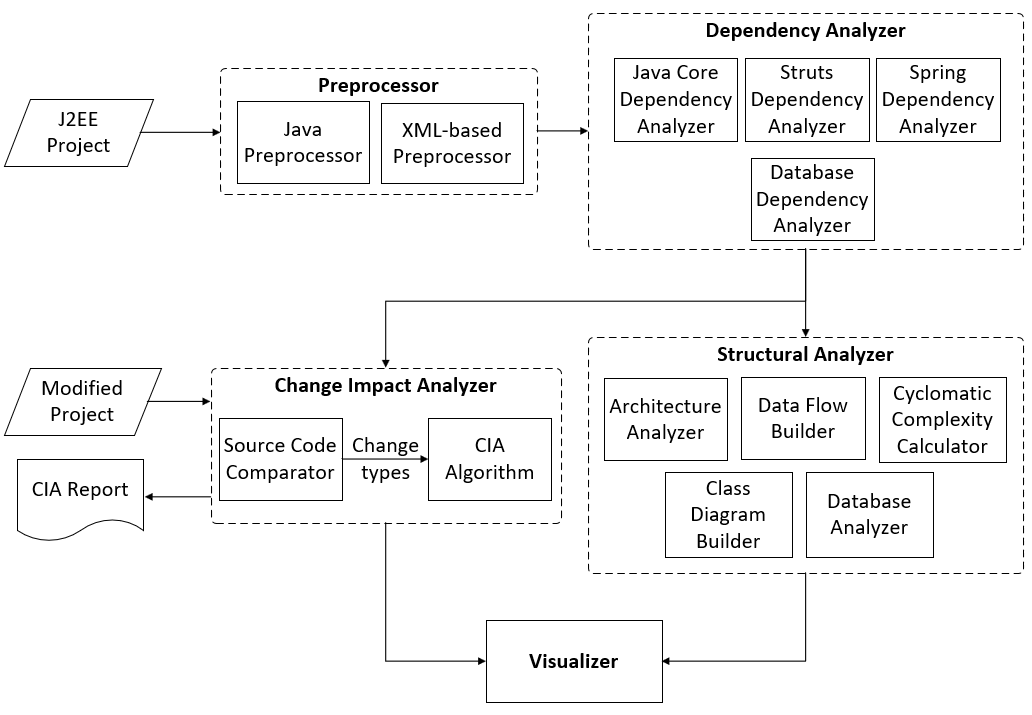
\includegraphics[scale=0.7]{jcia-vt-architecture}
	\label{fig:jcia-vt-architecture}
	\caption{Kiến trúc bộ công cụ JCIA-VT}
\end{figure}

Dựa trên những đề xuất phương pháp đã trình bày, bộ công cụ JCIA-VT được cài đặt bằng ngôn ngữ Java sử dụng framework Spring và được triển khai trên nền tảng ứng dụng Web. Bộ công cụ này nhận đầu vào là toàn bộ mã nguồn dự án doanh nghiệp sử dụng các nền tảng và công nghệ J2EE dưới dạng tệp nén. Bước đầu tiên toàn bộ mã nguồn sẽ được giải nén và tiền xử lý bởi mô-đun tiền xử cho Java và XML-based. Sau khi có được cây cấu trúc, mô-đun phân tích phụ thuộc sẽ làm nhiệm vụ tiếp theo: tương ứng với mỗi công nghệ framework sử dụng trong dự án sẽ có một bộ phân tích tương ứng làm nhiệm vụ phân tích phụ thuộc riêng. Kết thúc hai quá trình này, ta sẽ có cây cấu trúc cùng với các mối quan hệ phụ thuộc. Cây cấu trúc này có thể biến đổi làm đồ thị gọi cho thuật toán WAVE-CIA hoặc là đầu vào cho các mô-đun phân tích cấu trúc để xây các góc nhìn cho dự án.

Bước tiếp theo, để phân tích ảnh hưởng sử thay đổi, bộ công cụ yêu cầu người dùng tải lên một phiên bản của mã nguồn dự án. Bộ quản lý phiên sẽ thực hiện so sánh và phát hiện thay đổi, sau đấy tập các thành phần thay đổi được đưa vào thuật toán WAVE-CIA. Toàn bộ công việc này sẽ được mô-đun phân tích ảnh hưởng sự thay đổi thực hiện. Hoặc nếu trong trường hợp người dùng muốn sử dụng các bộ phân tích trong mô-đun phân tích cấu trúc. Các bộ phân tích này sẽ thực hiện trích xuất thông tin trên cây cấu trúc để xây dựng các góc nhìn về ứng dụng: góc nhìn kiến trúc công nghệ, dòng dữ liệu ứng dụng, biểu đồ lớp, sơ đồ liên kết thực thể, biểu đồ độ phức tạp mã nguồn.

Tất cả các kết quả phân tích đều có thể được hiển thị tới người dùng một cách trực quan nhờ mô-đun trình diễn. Mô-đun này được phát triển bằng Javascript sử dụng thư viện D3.js \footnote{  https://d3js.org}. Nó truy xuất và tương tác với dữ liệu của hệ thống phía sau bởi các API được cung cấp bởi Spring MVC.

\section{Thực nghiệm triển khai}

Hiện tại bộ công cụ đã được cài đặt và triển khai thực tế trên nền tảng Web tại địa chỉ \url{http://112.137.131.10:8080/jcia}. Bộ công cụ không yêu cầu người dùng cài đặt thêm bất cứ phần mềm nào, chỉ cần có một trình duyệt Web. Bộ công cụ cũng cho phép nhiều người dùng cùng sử dụng và phân tích đồng thời.

\subsection{Giao diện tải lên mã nguồn và phân tích phụ thuộc}
Sau khi đăng nhập thành công vào hệ thống bộ công cụ, ta sẽ được chuyển tới giao diện tải lên mã nguồn dự án và cấu hình các thông số cho việc phân tích như Hình \ref{fig:jcia-upload}. Tại giao diện ta ngoài việc chọn mã nguồn tải lên ở định dạng \textit{.zip}, ta cần phải quan tâm đến một số thông số như \textit{Java Source Path, Ignored Components, Analyzer(s)} và \textit{Node Level}.

\textit{Java Source Path} là đường dẫn tương đối dẫn đến thư mục chứa mã nguồn Java trong dự án J2EE. Ta cần cung cấp chính xác thông tin này bởi vì thư viện JDT cần biết nó cho việc đánh chỉ mục và xác định mối quan hệ cho các thành phần Java.

\begin{figure}[h]
	\centering
	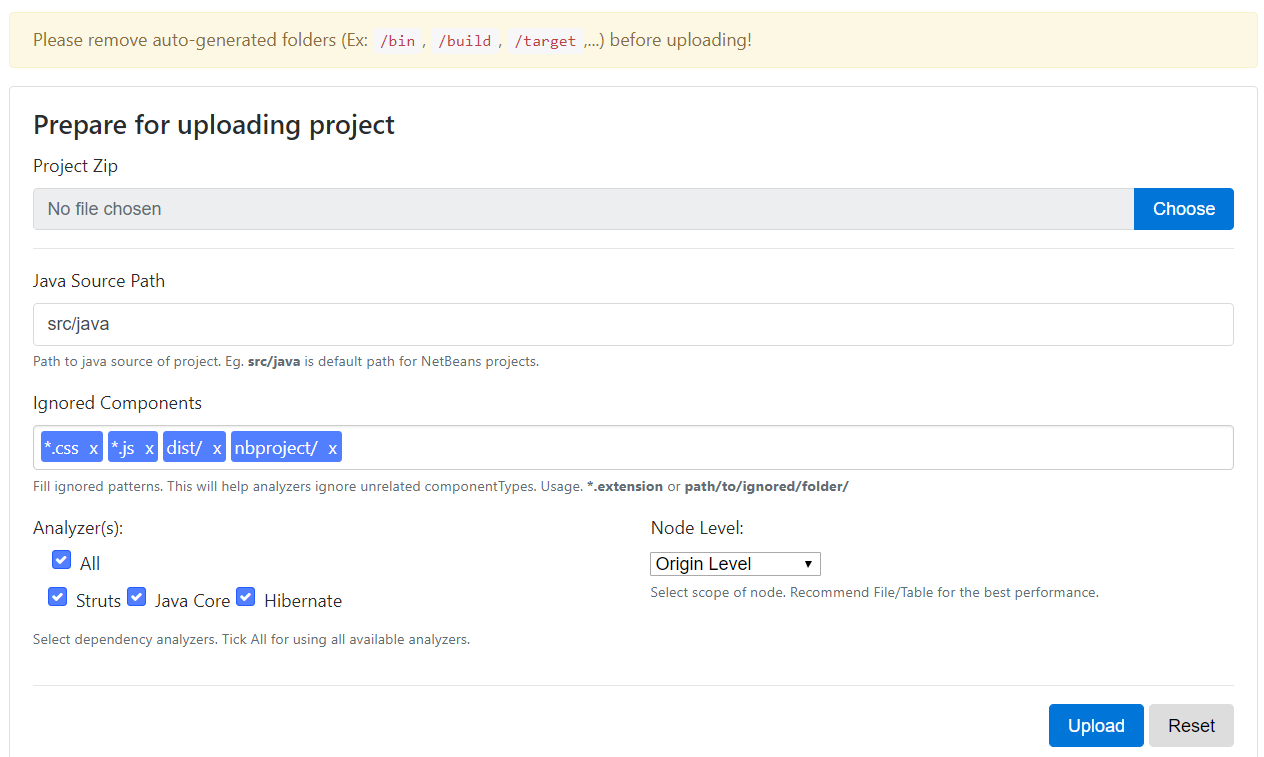
\includegraphics[width=0.9\linewidth]{jcia-upload}
	\label{fig:jcia-upload}
	\caption{Giao diện tải lên mã nguồn dự án}
\end{figure}

Trong toàn bộ mã nguồn dự án tải lên, có một số các định dạng mã nguồn bộ công cụ không hỗ trợ phân tích phụ thuộc như Javascript, CSS hay là các mã nguồn XML dùng cho việc lưu trữ thông tin cấu hình IDE khi người dùng phát triển mã nguồn (ví dụ với Netbeans IDE là toàn bộ mã nguồn trong thư mục \textbf{nbproject}). Nếu ta bỏ qua không phân tích những mã nguồn trên sẽ giúp tăng tốc độ thực hiện tiền xử lý và phân tích phụ thuộc. Ngoài ra, trong khi phát triển dự án, các nhà phát triển có thể đã thực hiện chạy thử dự án. Hoạt động này tạo ra các thư mục chứa các tệp nhị phân bytecode đã được biên dịch từ mã nguồn Java mà có thể chạy được, tuy nhiên một số tệp cấu hình sử dụng định dạng XML vẫn được giữ nguyên. Nếu các thư mục không được loại bỏ trước khi phân tích, thì sẽ có nhiều tệp cấu hình trùng tên với nhau khiến trình tìm kiếm không phân biệt và các mô-đun phân tích phụ thuộc sẽ không hoạt động chính xác. \textit{Ignored Components} được sử dụng cho mục đích loại bỏ các thành phần này không cần thiết trước khi phân tích, nó hỗ trợ hai kiểu là theo phần mở rộng (ví dụ: \textit{*.js, *.css}) và theo đường dẫn tương đối (ví dụ: \textit{dist/, nbproject/}).

Tùy chọn \textit{Analyzer(s)} cho phép người dùng chỉ định chính xác sẽ sử dụng những bộ phân tích phụ thuộc cho từng công nghệ cụ thể, hiện tại hỗ trợ cho Java Core, Struts và Hibernate. Tùy chọn \textit{Node Level} giúp người dùng lựa chọn độ sâu cho cây cấu trúc lúc hiển thị, độ sâu càng nhỏ thì lúc thao tác trên cây sẽ dễ dàng hơn. Tuy nhiên nó sẽ không hiển thị được chi tiết thông tin về các thành phần mã nguồn một cách đầy đủ nhất. Hiện tại có ba mức để lựa chọn là \textit{File/Table Level, Class/Table Level} và \textit{Origin Level}.

\subsection{Giao diện lịch sử phân tích và quản lý phiên bản}
\begin{figure}[h]
	\centering
	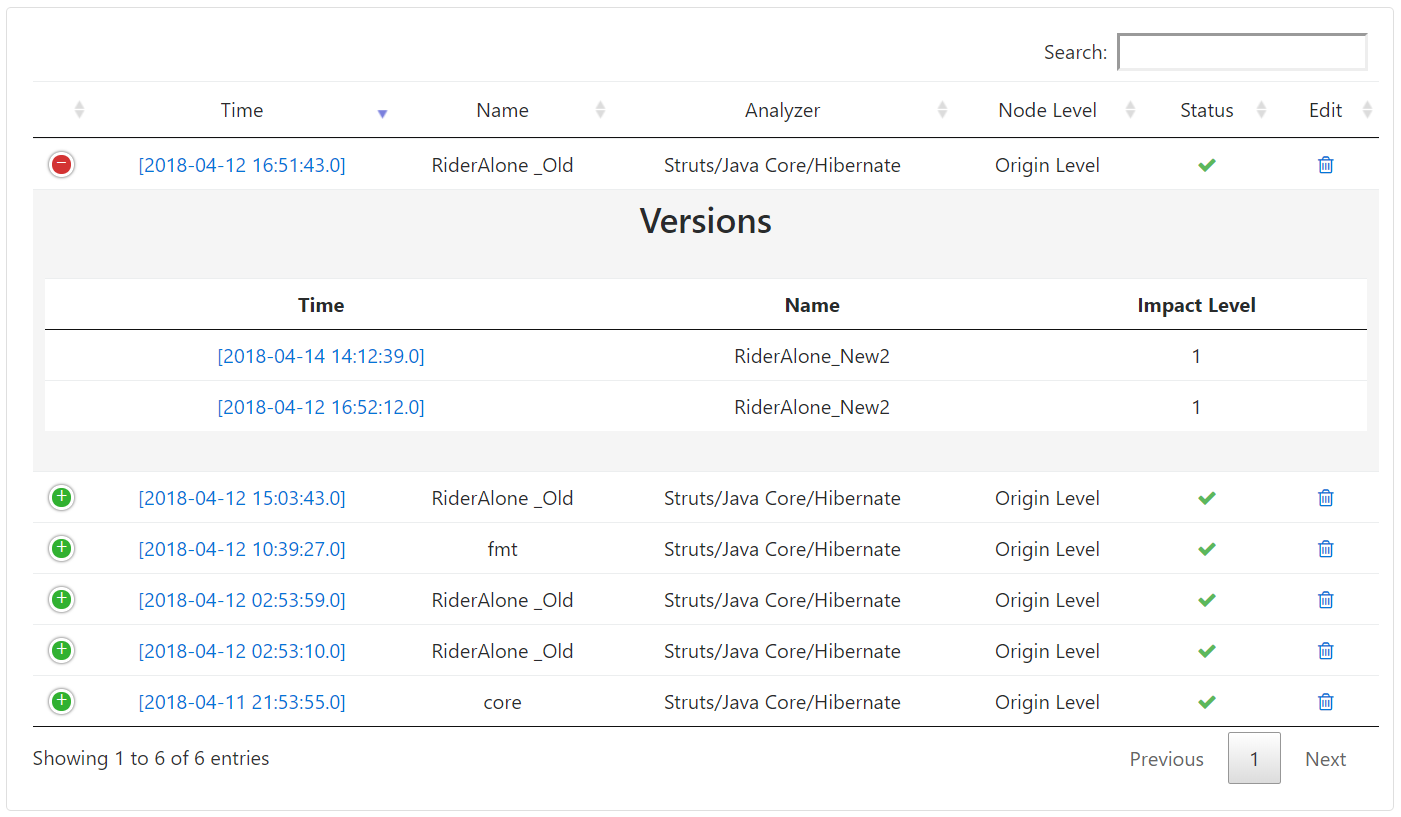
\includegraphics[width=0.9\linewidth]{jcia-history}
	\caption{Giao diện lịch sử phân tích quản lý phiên bản}
	\label{fig:jcia-history}
\end{figure}

Sau khi thực hiện tải lên và yêu cầu phân tích phụ thuộc cho dự án. Yêu cầu phân tích này sẽ được hệ thống đưa vào hàng đợi và thông báo về trạng thái tại giao diện lịch sử phân tích và quản lý phiên bản như Hình \ref{fig:jcia-history}.

Về tổng quan, giao diện này lưu trữ thông tin lịch sử phân tích (tên dự án, những bộ phân tích sử dụng và mức hiển thị nút) và các phiên bản cho các dự án được tải lên. Với dấu tích xanh ở trạng thái có nghĩa yêu cầu phân tích cho dự án đấy đã được thực hiện thành công. Nếu người dùng thực hiện cập nhật các phiên bản cho một dự án, chúng cũng sẽ được hiển thị ở giao diện này. Từ đây ta có thể theo dõi sự phát triển của dự án bằng các thông tin thay đổi qua các phiên bản cũng như thực hiện việc phân tích ảnh hưởng sự thay đổi khi so sánh hai phiên bản cụ thể của một dự án.

\subsection{Giao diện làm việc chính}
Tại giao diện lịch sử phân tích và quản lý phiên bản, sau khi ta thực hiện khôi phục lịch sự phân tích một dự án. Hệ thống sẽ đưa ta vào giao diện làm việc chính như Hình \ref{fig:jcia-workspace}.

\begin{figure}[h]
	\centering
	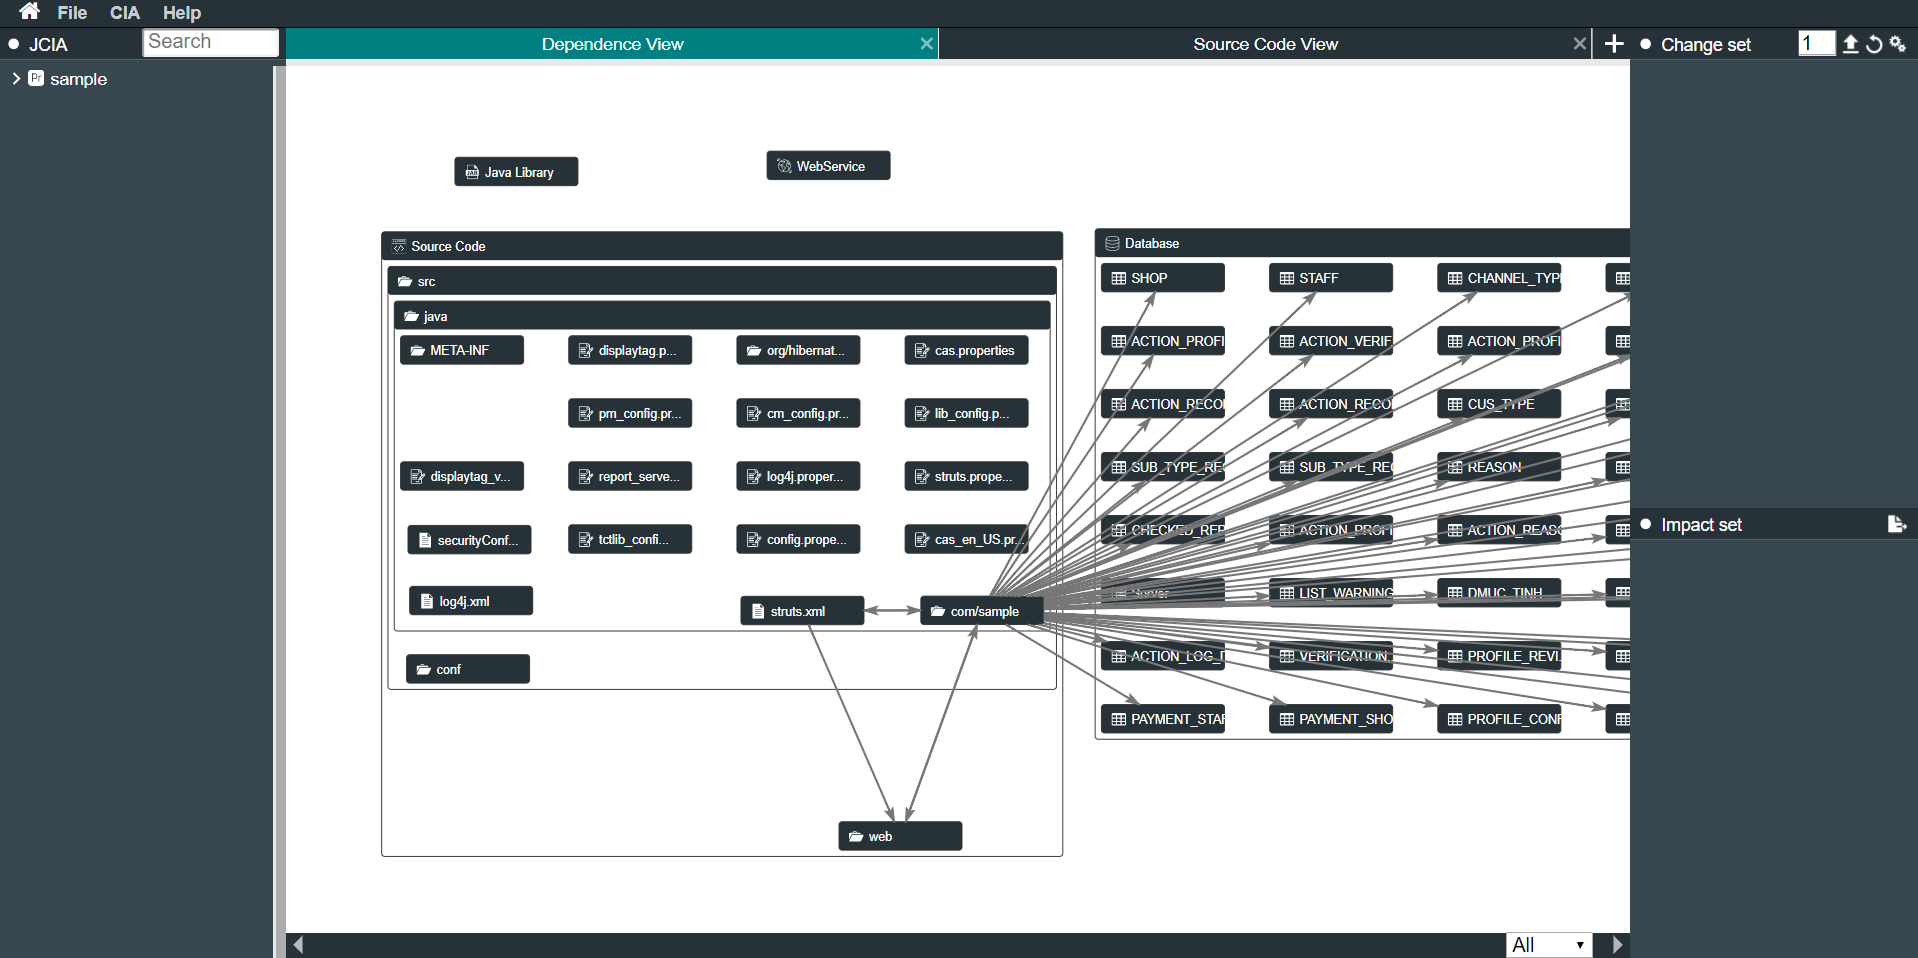
\includegraphics[width=1.0\linewidth]{jcia-workspace}
	\caption{Giao diện làm việc chính}
	\label{fig:jcia-workspace}
\end{figure}

Giao diện làm việc chính của bộ công cụ được chia làm bốn phần. Bên trái là khung nhìn theo dạng cây của dự án, cho phép ta duyệt và tìm kiếm nhanh các thành phần mã nguồn trên cây cấu trúc. Ở giữa là đồ thị phụ thuộc hiển thị các mối quan hệ phụ thuộc giữa các thành phần mã nguồn. Để xem chi tiết về thông tin các phụ thuộc của một thành phần, ta đưa trỏ chuột vào thành phần đấy, một bảng thông tin về các mối quan hệ phụ thuộc của nó sẽ hiện ra, ví dụ như Hình \ref{fig:jcia-workspace1} là thông tin các quan hệ phụ thuộc của \textit{struts.xml}.

\begin{figure}[h]
	\centering
	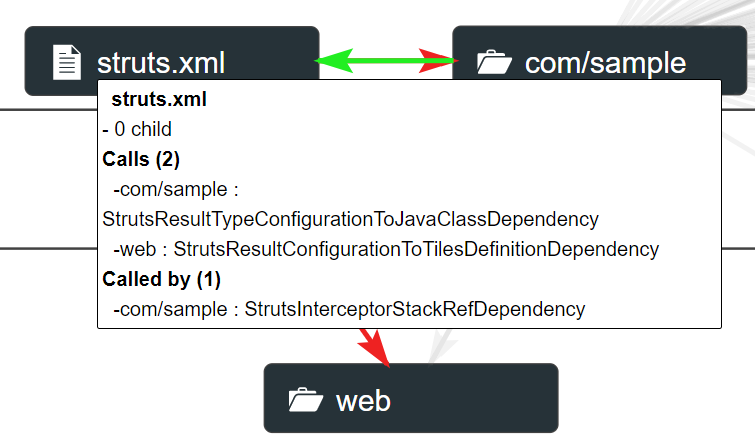
\includegraphics[width=0.6\linewidth]{images/jcia-workspace1}
	\caption{Ví dụ hiển thị mối quan hệ phụ thuộc}
	\label{fig:jcia-workspace1}
\end{figure}

\begin{figure}[h]
	\centering
	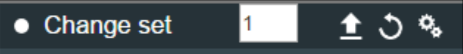
\includegraphics[width=0.5\linewidth]{images/jcia-workspace2}
	\caption{Các nút chức năng của Change Set View}
	\label{fig:jcia-workspace2}
\end{figure}

Phía bên trái giao diện chính gồm hai khung nhìn cho phục vụ cho việc phân tích ảnh hưởng sự thay đổi. Khung nhìn phía trên là hiển thị danh sách tập thay đổi. Tập thay đổi này được thu thập bằng cách so sánh các phiên bản của dự án, ngoài ra người dùng cũng có thể tự thêm vào bằng cách thao tác trên đồ thị phụ thuộc. Các nút chức năng của khung nhìn này ở Hình \ref{fig:jcia-workspace2}, cụ thể bao gồm:
\begin{itemize}
	\item \textit{Impact Level} là giá trị thể hiện mức lan ảnh hưởng được sử dụng trong thuật toán WAVE-CIA
	\item \textit{Upload Change Set} nếu muốn thay đổi nhiều nút cùng lúc, ta có thể tải lên
	một tệp text chứa đường dẫn của các nút thay đổi trong dự án. Công cụ sẽ tự tìm kiếm
	các nút đó và thêm chúng vào tập thay đổi.
	\item \textit{Clean All} xóa bỏ hết các tập thay đổi và tập ảnh hưởng đã phân tích
	\item \textit{Analyze} thực hiện phân tích tập thay đổi để tìm ra tập ảnh hưởng. Sau khi thực hiện phân tích ảnh hưởng thành công, khung nhìn ở giữa sẽ được chuyển sang đồ thị phụ thuộc mà trong đồ thị này chỉ có các nút có trong tập thay đổi và ảnh hưởng được hiển thị.
\end{itemize}

\subsection{Ví dụ minh họa}
\begin{figure}[h]
	\centering
	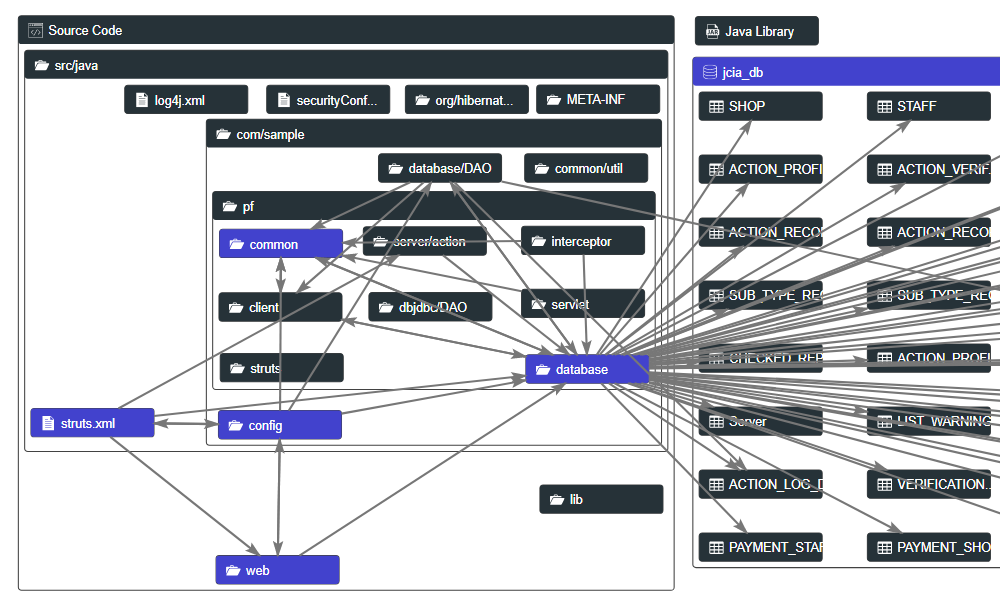
\includegraphics[width=0.8\linewidth]{images/sample-vitm}
	\caption{Ví dụ phân tích phụ thuộc cho dự án Struts thực nghiệm}
	\label{fig:sample-vitm}
\end{figure}

Hiện tại, bộ công cụ đã được triển khai thử nghiệm. Nhóm nghiên cứu sử dụng một dự án mẫu có sử dụng các framework Struts 2, Hibernate do tập đoàn Viettel cung cấp để làm dự án thực nghiệm. Phần này sẽ trình bày kết quả phân tích phụ thuộc mã nguồn, chạy thực nghiệm phân tích ảnh hưởng dựa vào kĩ thuật WAVE-CIA.

Sau khi thực hiện tiền xử lý và phân tích phụ thuộc cho dự án, hệ thống sẽ trả về cây cấu trúc kèm theo các phụ thuộc giữa các nút trên cây. Trên Hình \ref{fig:sample-vitm}, ta có thể thấy các phụ thuộc được biểu diễn bằng các mũi tên màu xám. Bộ tiền xử lý cho ta cây cấu trúc gồm thông tin về các thư mục và tệp trong mã nguồn dự án. Ta có thể thấy package \textit{common} là một package có nhiều mũi tên trỏ tới, bởi vì nó là một package Java được sử dụng nhiều trong dự án, điều này chứng minh rằng bộ phân tích phụ thuộc Java Core đã có hiệu quả nhất định. Ngoài ra, Bộ phân tích phụ thuộc cho Hibernate đã phân tích mã nguồn và xác định được tên các bảng trong CSDL và gán chúng lên cây cấu trúc, nhiều mũi tên xuất phát từ package \textit{database} tới các nút bảng cho ta thấy package \textit{database} là nơi chưa các lớp truy câp và thao tác trực tiếp tầng CSDL. Cuối cùng, những mũi tên giữa thư mục \textit{web, com/sample, config} và tệp \textit{struts.xml} là kết quả của bộ phân tích Struts 2. Các mũi tên từ \textit{struts.xml} và \textit{config} tới package \textit{com/sample} thể hiện cho sự phụ thuộc của các định nghĩa \textit{Action, Interceptor, Result Type} bằng các lớp Java; tới thư mục \textit{web} thể hiện cho sự phụ thuộc các định nghĩa \textit{Result}.

Bộ công cụ cung cấp hai cách để thực hiện việc phân tích ảnh hưởng sự thay đổi. thứ nhất là người dùng chọn tập thay đổi và phân tích trực tiếp trên giao diện hiển thị phụ thuộc, thứ hai là phân tích tự động bằng cách người dùng tải lên mã nguồn đã thay đổi, công cụ thực hiện so sánh hai phiên bản mã nguồn và phân tích ảnh hưởng rồi trả về báo cáo kết quả.

\begin{figure}[h]
	\centering
	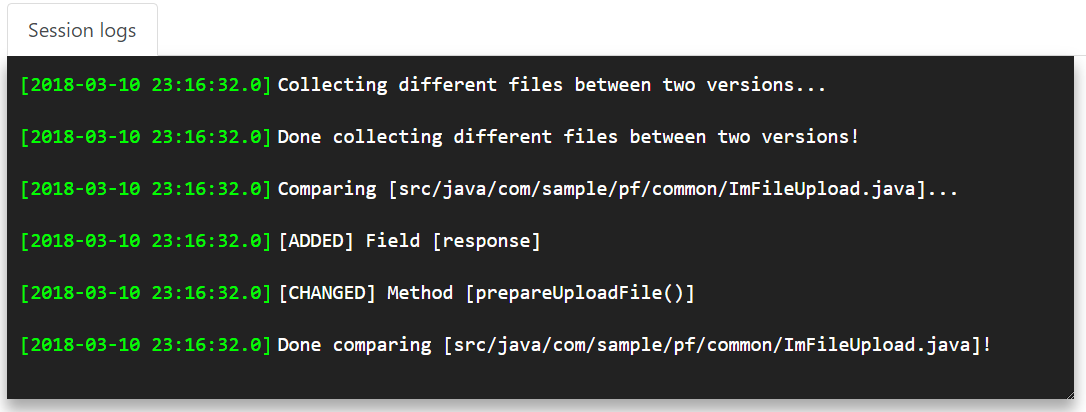
\includegraphics[width=0.8\linewidth]{images/sample-vitm-1}
	\caption{Ví dụ phân tích phụ thuộc cho dự án Struts thực nghiệm}
	\label{fig:sample-vitm-1}
\end{figure}

\begin{figure}[h]
	\centering
	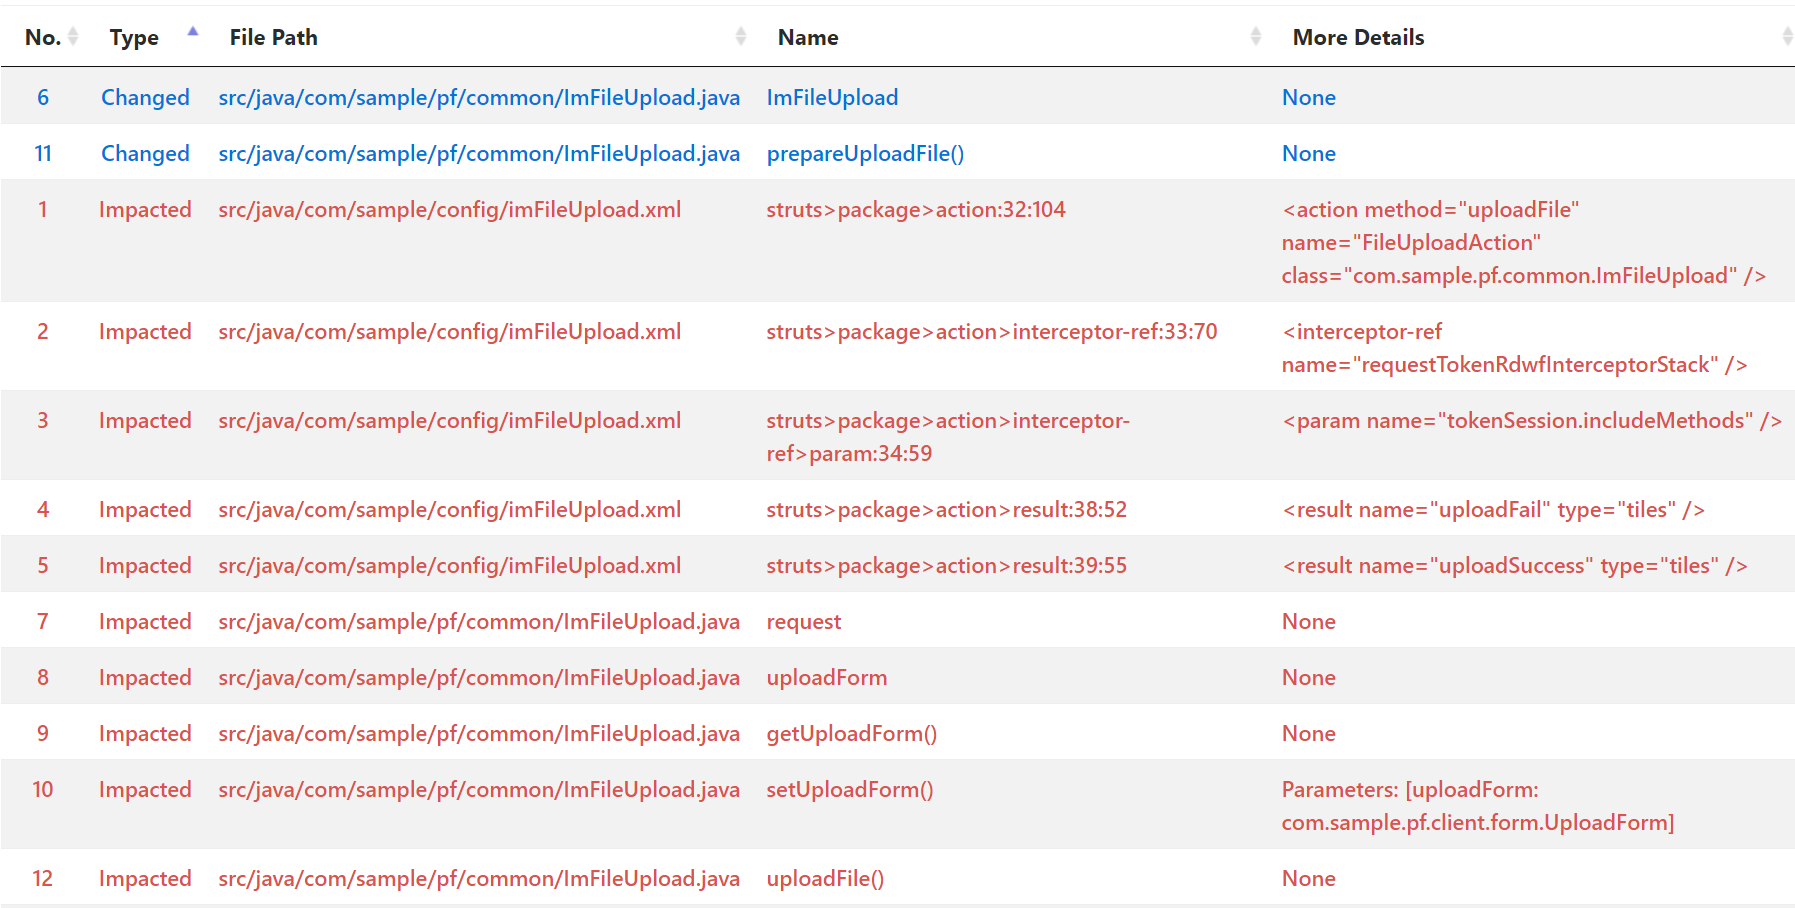
\includegraphics[width=0.9\linewidth]{images/sample-vitm-2}
	\caption{Ví dụ phân tích phụ thuộc cho dự án Struts thực nghiệm}
	\label{fig:sample-vitm-2}
\end{figure}

Hình \ref{fig:sample-vitm-1} và Hình \ref{fig:sample-vitm-2} lần lượt biểu diễn cho nhật ký hoạt động và kết quả của quá trình phân tích ảnh hưởng sự thay đổi sử dụng bộ so sánh phiên bản cho một ví dụ cụ thể. Với giả định cải tiến cho chức năng \textit{Upload File} của dự án mẫu, chúng tôi đã thực hiện bằng cách thêm thuộc tính \textit{response} và thay đổi phương thức \textit{prepareUploadFile()} trong tệp \textit{ImFileUpload.java}. Sau khi mã nguồn mới được tải lên, bộ so sánh phiên bản được thực thi, công cụ đã phát hiện chính xác các thay đổi giữa hai phiên bản, ta có thể thấy trong nhật ký so sánh ở Hình \ref{fig:sample-vitm-1}. Tiếp theo, bộ phân tích ảnh hưởng được thực hiện với tham số mức độ ảnh hưởng là 3 cho ta kết quả như Hình \ref{fig:sample-vitm-2}.

\chapter{Kết luận}
Nghiên cứu này đã đề xuất các phương pháp và bộ công cụ phục vụ cho các hoạt động đảm bảo chất lượng mã nguồn các ứng dụng doanh nghiệp trên nền tảng và công nghệ J2EE. Ở giai đoạn này, chúng tôi đã hoàn thành cơ bản các chức năng chính của bộ công cụ nhằm đáp ứng cho việc phân tích mã nguồn các ứng dụng sử dụng Struts 2 và Hibernate. Dựa trên những gì đã thực hiện được, trong giai đoạn tiếp theo, sẽ có thêm nhiều phụ thuộc được thêm vào để xử lý giúp bộ phân tích ảnh hưởng dự đoán tập ảnh hưởng chính xác hơn. Bộ quản lý vào so sánh các phiên bản mã nguồn sẽ được tích hợp với các hệ thống quản lý phiên bản hiện nay như Git  và SVN . Điều này giúp cho việc thực hiện phân tích ảnh hưởng và báo cáo kết quả hoàn toàn tự động mà không cần đến các thao tác của con người. Đây cũng là một lợi thế để áp dụng các kĩ thuật CIA có tính chính xác cao hơn như kĩ thuật CIA dựa vào phân loại thay đổi bởi bộ so sánh phiên bản có thể xác định chính xác từng loại thay đổi trên các thành phần mã nguồn. Đối với các kiểm thử viên, chức năng phân tích ảnh hưởng có thể giúp họ chỉ cần thực hiện một số ca kiểm thử nhất định khi có đội phát triển thay đổi mã nguồn. Tuy nhiên, hiện nay hầu hết các ca kiểm thử được thực hiện dựa trên các tài liệu biên bản kiểm thử mà chúng mô tả các bước kiểm thử bằng tay trên giao diện ứng dụng chứ không phải tự động bằng Unit Test. Trong khi đó kết quả của bộ phân tích ảnh hưởng là các thành phần mã nguồn, do đó một bộ ánh xạ giữa thành phần mã nguồn và các màn hình hoặc chức năng ứng dụng cần được tích hợp để bộ công cụ này thực sự có ích và có thể ứng dụng đại trà vào quá trình đảm bảo chất lượng cho nền công nghiệp phát triển phần mềm ở các công ty hiện nay. Ngoài ra, cần có thêm nhiều góc nhìn về ứng dụng cần được tích hợp để người sử dụng thêm nhiều thông tin cho ứng dụng của mình như biểu đồ tuần tự giữa các package, biểu đồ dòng điều khiển và các công cụ đánh giá về độ phức tạp mã nguồn và bảo mật của ứng dụng, v.v. Bộ công cụ sẽ hỗ trợ cho thêm nhiều công nghệ và nền tảng khác của Java, và xa hơn nữa, nhóm sẽ nghiên cứu để bộ công cụ có thể phân tích cho các ngôn ngữ khác như C\#, PHP, Javascript.
\end{document}
